\documentclass[9pt,conference]{IEEEtran}

\usepackage{cite}
\usepackage{amsmath,amssymb}
\usepackage{booktabs}
\usepackage{graphicx}
\usepackage{algorithm}
\usepackage{algorithmic}
\usepackage[T1]{fontenc}
\usepackage[utf8]{inputenc}

\def\BibTeX{{\rm B\kern-.05em{\sc i\kern-.025em b}\kern-.08em T\kern-.1667em\lower.7ex\hbox{E}\kern-.125emX}}


% ---- density settings, injected by make_variants.py; edit that, not this file ----
\usepackage[margin=0.25in]{geometry}
\linespread{0.85}
\setlength{\parskip}{0pt}
\setlength{\columnsep}{0.10in}
\setlength{\textfloatsep}{3pt}
\setlength{\floatsep}{3pt}
\setlength{\intextsep}{3pt}
\setlength{\abovedisplayskip}{3pt}
\setlength{\belowdisplayskip}{3pt}
\setlength{\abovecaptionskip}{3pt}
\setlength{\belowcaptionskip}{3pt}
\usepackage{microtype}
\usepackage[compact]{titlesec}
\titlespacing*{\section}{0pt}{3pt}{2pt}
\titlespacing*{\subsection}{0pt}{3pt}{1pt}
\usepackage{enumitem}
\setlist{nosep,leftmargin=*}
% fontsize rescales the whole ladder -- \small, \footnotesize and the tables with it --
% which a bare \fontsize does not, and which would leave table text larger than body text.
\usepackage[fontsize=7.0pt]{fontsize}
% ---------------------------------------------------------------------------------

\begin{document}

\title{How Generous You Already Are Predicts\\
Whether Fairness Gives or Takes}

\author{\IEEEauthorblockN{Dheirav}
\IEEEauthorblockA{\textit{Responsible AI} \\
\textit{Algorithmic Bias Mitigation}\\
\texttt{dheirav2005@gmail.com}}}

\maketitle

\begin{abstract}
A group-fairness constraint requires two groups' selection rates to be close, but it does not
say how the gap should close: the disadvantaged group can be lifted, or the advantaged group
can be pulled down. Both outcomes satisfy the constraint, and the certifying metric is
content with either --- it reads \textbf{0.018} where the constraint destroyed a fifth of
the favourable decisions and \textbf{0.010} where it created more than it destroyed, so a
team cannot tell from its own dashboard which it is about to cause. We show the direction is
a property of the \emph{population} rather than of the method, predictable in advance from a
quantity every deploying organisation already has: the rate at which its current model says
yes, read against that population's crossover. Across 161 disjoint population samples covering six decision domains
and eight data sources on five countries, an attribute-blind constraint withdraws below a
population's crossover and extends above it; on UCI Adult five in-processing methods each shrink the pool by
7.9--22.1\%, while on mortgage lending the identical constraint grows it. The practical output is an
audit that locates a team's own crossover and \emph{refuses} when it cannot: on fifty
populations drawn at random, frame and seed fixed in advance, 78\% admit a directional rule
and 22\% do not, and the procedure returns the latter as unanswerable rather than scoring
them.

The claim is deliberately narrow, and sealed tests made it so. \textbf{Direction is
predictable within a population; magnitude is not}, and a sealed model of it lost to
predicting zero; below one percentage point the direction call is 61\% correct, which is a
coin flip. Which quantity carries the prediction was settled by elimination under
seal: a screen-gated Brazilian race cohort separated the rate from label rarity in the
rate's favour, and a sealed lending cohort beat a loan-purpose null on real approvals. Crossovers are population-specific --- located values span 0.28 to 0.65 ---
so a fixed prior is a fallible substitute for measuring one's own: the rule sealed at
\textbf{9 of 10} on never-measured populations (best constant 6; binomial tail 0.046
against a guesser, but only $p \approx 0.19$ paired against that constant), while the specific
value 0.54 scored 5 of 10 on a second cohort and holds no privilege over 0.50. Of nine
sealed or registered direction tests, one passed; we report the failures because each
removed a stronger claim than the one that survives. The relationship survives changes of
route, tolerance, base learner and protected attribute, but disappears under post-processing --- a sealed test locating that
boundary at the optimizer family, not attribute access. One scope limit belongs here:
\textbf{in five of the eight sources the favourable decisions are predicted labels rather
than allocations}, and HMDA, the one source recording real approvals, is where our sweep
protocol failed its held-out test.
\end{abstract}

\begin{IEEEkeywords}
algorithmic fairness, levelling down, demographic parity, in-processing, selection rate,
disparate impact
\end{IEEEkeywords}

\section{Introduction}

A fairness constraint says that two groups' rates should be close, but it does not say how
that closeness should be reached. The gap can close because the disadvantaged group is
lifted, or because the advantaged group is pulled down, and while both directions satisfy
the constraint, they are morally very different outcomes on most --- though, we note, not
all --- accounts of what the constraint is for; at minimum, anyone imposing one deserves
to know which they are getting.

This ambiguity is already well established. Mittelstadt \emph{et al.} \cite{mittelstadt2023}
made levelling down the centre of a well-known critique; Maheshwari \emph{et al.}
\cite{maheshwari2023} observe that it ``often goes unnoticed in the overall performance of
the model''; and Krco \emph{et al.} \cite{ferry2023} built an auditing framework precisely
because an aggregate score reports neither how many people were affected nor in which
direction. We take all of that as given.

What the literature leaves open is the question a deploying team actually faces:
\textbf{when} does each direction happen? The question is not academic, because the
certifying number is not merely silent about the answer --- it is equally content with
either. On UCI Adult a demographic-parity constraint destroyed roughly a fifth of the
favourable decisions, and the parity difference it was certified against read
\textbf{0.018}. On HMDA mortgage data the identical constraint created more favourable
decisions than it destroyed, and the parity difference read \textbf{0.010}. Both pass. A
team looking only at its fairness dashboard cannot tell which of the two it has just done.

\textbf{The claim, in one sentence.} Whether a parity constraint hands out more favourable
decisions or takes them away is a property of the \emph{population} being decided about
rather than of the fairness method --- and a team can measure which one it is about to
cause, before it causes it, from the rate at which its current model already says yes.

The audit that follows from it has \emph{three} outcomes rather than two --- the constraint
will give, it will take, or the population admits no answer and the audit says so
(Algorithm~\ref{alg:locate}). The third is not a caveat attached to the method; it is a third
of what the method does.

Four conditions bound the sentence above. Each is measured rather than assumed, and each was
bought with a test that failed:

\begin{itemize}
\item \textbf{Direction only, and only above a floor.} A sealed model of magnitude lost to
predicting zero (MAE 4.50 against 0.77). Effects below one percentage point are called
correctly 61\% of the time --- a coin flip --- against 95\% above it.
\item \textbf{About four populations in five.} On fifty populations drawn at random, frame
and seed fixed before any arm ran, 78\% admit a directional rule and 22\% do not. The
procedure \emph{refuses} the 22\% rather than guessing at them.
\item \textbf{In-processing, not post-processing.} Under post-processing the relationship is
absent ($r = -0.024$), and a sealed deconfounding test locates that boundary at the
optimizer family rather than at access to the protected attribute
(Section~\ref{sec:regime}).
\item \textbf{Mostly predicted labels, not allocations.} In five of the eight data sources
the favourable decisions are model predictions rather than decisions actually made. HMDA,
the one source recording real approvals, supports the direction claim on its natural arms
but is also where our sweep protocol failed its held-out test.
\end{itemize}

The rule underneath is not surprising once stated: say yes often and the constraint tends to
give, say yes rarely and it tends to take. What is \emph{not} available without measuring is
where the boundary falls for a particular population. Located crossovers span 0.28 to 0.65.
In the one setting where we drew populations at random rather than choosing them --- US
state-level income prediction, fifty draws --- no population's operating rate reached 0.55,
and 25 of the 47 with a computable rate sat inside that 0.28--0.65 span, which is precisely
where an unaided reading of ``often'' against ``rarely'' has nothing to say. A further fifth
of them follow no directional rule at all; there the intuition still returns a confident
answer, and the audit declines to.

\subsection{Scope, stated first}
\label{sec:scope}

This is a paper about \textbf{attribute-blind in-processing} constraints, meaning the regime
in which the protected attribute is unavailable at decision time. This is the regime most
deployed systems occupy: in the United States, per-group decision thresholds face direct
disparate-treatment exposure (\emph{Ricci v.\ DeStefano} \cite{ricci2009}; in credit, ECOA
and Regulation B prohibit attribute-based terms outright), and commentators read the
doctrine the same way \cite{barocas2016,corbett2017}. Two honest qualifications. First,
the barrier is jurisdiction-specific, and the two major jurisdictions draw it in different
places: in the US even \emph{training-time} use of the attribute --- which every
in-processing method here involves --- is legally unsettled, while in the EU the split
runs the other way: \emph{decision-time} use of special-category data faces GDPR
Article~9 and direct-discrimination doctrine, but training-time use for bias detection
and correction in high-risk systems is expressly permitted, under safeguards, by
Article~10(5) of the AI Act --- and for race and ethnicity the blind regime is often
simply factual, because most member states collect no such attribute at all. Second,
because of that split we motivate the regime as the one systems occupy, not as one any
law cleanly compels. Under
post-processing the effect we report disappears, and a sealed deconfounding test shows
the disappearance belongs to the method, not to the attribute: the same in-processing
optimizer, given the attribute, preserves the relationship
(Section~\ref{sec:regime}). The blind regime remains the paper's scope because it is
where the record was built and where deployed systems sit --- not because blindness is
what the finding depends on.

\subsection{Contributions}

The list is ordered by how much weight each item carries. The first two are the paper; the
rest defend, bound, or record them.

\begin{enumerate}
\item \textbf{The phenomenon, measured at scale.} An attribute-blind parity constraint
withdraws favourable decisions on some populations and extends them on others, and the
certifying metric reports the same kind of number in both cases. On UCI Adult five
in-processing methods each shrink the pool by 7.9--22.1\%, at an exchange rate of 2.68
decisions destroyed per one created; on HMDA mortgage lending the identical constraint grows
it by 4.3\%, at an exchange rate of 0.50. Measured across \textbf{161 disjoint population
samples} spanning six decision domains, eight data sources and five countries. Rates
understate this: measured in \emph{people} rather than rates, between 0.66 and 0.74 of those
whose decision changed are advantaged-group members losing a favourable one, and the
divergence between the two views is itself predictable ($r = +0.885$).

\item \textbf{An audit that answers for one's own population --- and refuses when it
cannot.} The same design that produced the record lets a practitioner locate their own
crossover from their deployed model; three overlapping estimates of the mortgage crossover
agree, all from one two-state market. The refusal is not a caveat but half the contribution.
How often a parity constraint's response is even \emph{shaped} so that a directional rule
can apply had not been measured: on fifty populations drawn at random, frame and seed fixed
before any arm ran, 78\% admit one and 22\% do not, of which 64\% are classic
single-crossing landscapes. The procedure returns those 22\% as unanswerable rather than
scoring them, which is what separates it from reading a number off a dashboard --- detecting
a non-monotone landscape requires the sweep that transporting a prior exists to avoid
(Section~\ref{sec:boundaries}).

\item \textbf{The predictor identified by elimination, not by assertion.} Varying the
selection rate by moving a label threshold cannot alone distinguish ``the rate predicts''
from ``task difficulty does''; holding the task fixed and moving only the decision rule
separates them across the mid-range. Three further alternatives were ruled out under seal.
A screen-gated Brazilian race cohort --- ten arms from two person-samples, so the confound
is broken \emph{within} populations rather than across them --- \textbf{broke the
cutoff-versus-rate confound in the rate's favour}: on mixed-route sealed arms the
cutoff-only reading scored 5 of 10 against the rate rules' 8--9, and the selection rate,
not label rarity, carries the prediction. A sealed lending cohort beat a purpose-only null
8 vs 5 on real approvals, so the loan product does not carry it either. A five-domain
comparison rules out the group gap. We say \emph{predicts}, never \emph{causes}: no pooled
slope transfers across populations (Section~\ref{sec:boundaries}).

\item \textbf{An empirical characterisation of a conditionality that theory predicts.}
Contemporaneous theory \cite{backfire2026} establishes that in the attribute-blind regime
the direction is distribution-dependent. It contains no experiments and its conditions are
ordering relations on score regions rather than measurable quantities. We supply the
measurement, and find that a percentile-relaxed form of the theory's ordering agrees with
the measured direction on 24 of 26 arms and correlates with our predictor at $r = +0.935$:
the selection rate operationalizes the theory's quantity. That correspondence has since been
stress-tested: it holds across 150 \emph{arms} --- population-label pairs in the sense of
Section~\ref{sec:setup}, not independent populations, several of which contribute an arm at
more than one cutoff --- with $r = +0.850$ (population-clustered bootstrap 95\% interval
$+0.813$ to $+0.892$), is invariant to the trim percentile, survives a gradient-boosted
second probe ($r = +0.946$), and on the sealed cohorts head-to-head the rate calls 18 of 19
to the relaxed ordering's 17. The exact conditions --- \emph{sufficient, not necessary} ---
were certified on zero of the 26 by our logistic-probe plug-in, whose ratio diverges in the
$\hat\nu$ tail: an estimator pathology, not a property of the conditions, and we tried no
other estimator (Section~\ref{sec:regime}).

\item \textbf{Two predictive claims, distinguished by what they require --- and a fixed
prior demoted to its measured failure rate.} The paper contains a \emph{sweep-conditional}
claim --- run the audit on your own data and, where the response is monotone, the rate
against your own measured crossover predicts direction --- and a weaker
\emph{transported-prior} claim, the only one testable before any measurement. The direction
rule itself is \emph{sealed}: committed before ten populations this work had never measured,
it scored 9 of 10 against a best constant of 6 (Section~\ref{sec:resealed}), and the
within-population claim passed sealed off-instrument on Brazil. The fixed \emph{value} 0.54
fares worse and we no longer present it as a finding. Crossovers are population-specific,
located values spanning 0.28 to 0.65; the value failed its own strict bar on the race cohort
(a 0.50 prior edged it by one arm in-band), and on a second, post-hoc cohort of larger
states it scored 5 of 10 --- each miss agreeing with that population's own measured
crossover. It is a fallible substitute for measuring, with a failure rate we can quote, and
sweeping the arms where it fails shows they are populations with \emph{no} directional rule
to get right rather than populations where the rule got it wrong. The procedure refuses all
of them; only the prior is exposed.

\item \textbf{Boundaries stated explicitly rather than left for review to find}, including a
computable test for when the procedure cannot be used at all. Of nine sealed or registered
direction tests, one passed; we report the failures because each removed a stronger claim
than the one that survives, and because a cohort built to strengthen the paired statistic
showed the attempt is self-defeating --- the magnitude guard such a test requires deletes
the near-crossover arms it needs. The relationship survives a change of route, a
twenty-five-fold tolerance range, a boosted-tree learner and a protected attribute swapped
from sex to race, but disappears under post-processing.
\end{enumerate}

\section{Related Work}

\textbf{Whether levelling down is universal.} A 2026 theory paper \cite{backfire2026} proves in
a population-level Bayes framework that the answer depends on the deployment regime. Where the
protected attribute is available at decision time, fairness ``necessarily (weakly) improves
outcomes for the disadvantaged group and (weakly) worsens outcomes for the advantaged group''.
Where it is not --- the attribute-blind regime, which is ours --- ``the impact of fairness is
distribution-dependent: fairness can benefit or harm either group $\ldots$ leading to either
leveling up or leveling down.'' \textbf{We therefore do not claim the conditionality itself.}

\textbf{Levelling down, and the remedy.} Mittelstadt \emph{et al.} \cite{mittelstadt2023} argue
that fairness interventions frequently equalise by degrading the better-off group, and
\emph{also propose the remedy}: minimum rate constraints requiring ``that every group has, at
least, a minimal selection rate, precision, or recall''. We claim neither the observation nor
the remedy as novel. Our contribution relative to that work is narrow and checkable: a scope
condition they do not have; in-processing rather than post-processing, so no model reads the
attribute when predicting; a population-level floor stacked \emph{with} parity rather than a
per-group floor replacing it; and held-out replication where they report training-set results.

\textbf{Auditing individual impact.} Krco \emph{et al.} \cite{ferry2023} propose a framework
whose first three dimensions are impact size, change direction and decision rates. That is the
decomposition we use throughout, and we claim no part of it. What we add is what those axes
report at scale: the change-direction dimension is not a property of the method being audited
but of the population it is applied to.

\textbf{The shape of the optimal fair classifier.} Corbett-Davies \emph{et al.}
\cite{corbett2017} show that for several fairness definitions the optimal constrained
classifier takes the form of group-specific risk thresholds. This gives a \emph{bound} rather
than another baseline: it predicts that levelling down is not an artifact of the reduction's
search, because the optimal constrained classifier withdraws in the same way.

\textbf{Remedies that avoid harm.} Minimax group fairness \cite{diana2021} minimises the worst
group's error rather than equalising anything, and is the natural alternative to a parity
constraint for a team whose concern is harm rather than equality. We benchmark against it
rather than only against the unconstrained reduction.

\textbf{The selection-rate axis.} The nearest prior work is Goethals \emph{et al.}
\cite{goethals2024}, which studies the cost of fairness as a function of available budget and
reports that ``the level of available resources significantly influences this cost, a factor
overlooked in prior evaluations''. The difference is structural: in their setting positive
decisions are a fixed resource, so the total is constant by construction and the directional
effect we measure cannot arise.

\textbf{Fairness gerrymandering and dataset monoculture.} Kearns \emph{et al.}
\cite{kearns2018} show constraints on marginal groups can be satisfied while subgroups are
badly treated. Ding \emph{et al.} \cite{ding2021} argue the field should stop drawing
conclusions from UCI Adult and supply ACS-derived replacements. Notably they also
\emph{build the knob this paper turns}: the \$50{,}000 threshold ``was chosen so that this
dataset can serve as a replacement to UCI Adult, but we also offer datasets with other income
cutoffs''. They do not connect it to the direction of a fairness intervention --- their text
contains no occurrence of ``selection rate'', ``acceptance rate'' or ``leveling down'' --- so
the instrument existed and the question was not asked of it. We replicate across their
populations and then find that is \emph{not sufficient}, because they share one survey
instrument.

\section{Setup and Method}
\label{sec:setup}

\textbf{Data.} 161 independent populations across eight data sources.
Two are US surveys: UCI Adult (45{,}222 rows), and ACS Income \cite{ding2021} across
102 state-years --- forty-two at 2018, twenty-five at 2014, thirty-one at 2019 and four at
2022 --- and two protected attributes. One records real allocations: HMDA 2018 mortgage
filings for \textbf{every state in the country} (Mississippi and Louisiana throughout the record; Alabama,
South Carolina, Tennessee, Georgia, North Carolina and Ohio added for the six-market seal;
eight more for the sealed lending cohort of Section~\ref{sec:failures} and eight scored
post-hoc beside it; 30{,}000--305{,}593 records each). The remaining five are
IPUMS International census extracts for Brazil (2000, 2010) and Mexico (2015, 2020), sex
arms, labels set by income quantile with the loader's filter and 60{,}000-row sealed
subsamples per population (Section~\ref{sec:resealed}); COMPAS \cite{propublica2016}
(5{,}278 rows on the race arm after ProPublica's documented filter); LSAC bar passage
(20{,}798 rows); the Dutch national census of 2001 (60{,}420 rows); and Taiwanese
credit-card default records of 2005 (30{,}000 rows). A
\emph{population} here is one such unit --- a state, cohort or census --- and
\emph{independent} means disjoint person samples: no person appears in two of them, and
arms within a population share people, so however many arms a population contributes, it
is counted once (Table~\ref{tab:accounting}); the eight data sources remain the honest
count of independent \emph{instruments}. Three survey-methodology conventions are
deliberate and inherited from the folktables benchmark \cite{ding2021}: ACS person records
are used \emph{unweighted} (no \texttt{PERWT}), incomes are nominal \texttt{PINCP} without
the \texttt{ADJINC} adjustment, and household clustering is not modelled, so every
``selection rate'' here is a property of the unweighted sample rather than a
design-consistent state estimate. The weighted re-analysis has since run: read under
PWGTP, every located crossover shifts \emph{down} by 0.03--0.08 in weighted rate units
while the ordering and the two outliers are unchanged --- so the numeric locations,
including the 0.54 prior, are properties of this convention, stated as such where they
appear, while the audit itself needs no weights (a deployer's held-out pool is the
population of interest). Seed-resampled intervals are anti-conservative, and a
household-clustered bootstrap widens the sex-arm intervals modestly (South Carolina
0.470--0.587 against 0.454--0.537 person-resampled) without dislodging any location.
Two further PUMS facts bound what the labels can mean: state topcodes sit far above
every cutoff used here, so topcoding is benign; a fifth or more of PUMS incomes are
hot-deck imputations, a share that rose in pandemic vintages, and the allocation screen
has since run: excluding flagged rows lifts base rates by about $+0.03$
\emph{uniformly} --- both vintages, both labels, gaps stable, directions preserved ---
so imputation is a level effect everywhere and is acquitted as a differential 2022
mechanism, the fourth candidate cleared.

\textbf{The lending outcome, defined.} On HMDA the outcome is the \emph{lender's}
approval: action-taken codes 1 (originated) and 2 (approved, not accepted) against 3
(denied), with withdrawn, incomplete, purchased and preapproval records excluded as not being
a completed approve-or-deny. Features are restricted by allow-list to what exists when the
application is filed. The race arm is White vs.\ Black applicants, the sex arm Male vs.\
Female (joint applications excluded), and loan purposes are sub-populations.

COMPAS, LSAC and the Dutch census were added to leave the sources the finding was formed
in. The Dutch census
carries a between-group gap of 0.298, roughly twice Adult's, making it the test of the standard
alternative explanation. LSAC was chosen because bar passage is naturally generous (base rate
0.890).

\textbf{Definitions, in one place.} An \emph{arm} is one population under one
configuration (a decision threshold, a label cutoff, a tolerance, a learner). The
\emph{selection rate} $r$ is the fraction of the test split the baseline model marks
favourable. The \emph{pool change} $\Delta$pool is the percentage change, baseline to
mitigated, in the number of favourable decisions; \emph{up}/\emph{extension} and
\emph{down}/\emph{withdrawal} name its sign. A population's \emph{crossover} is the rate
at which its pool change changes sign, reported as the bracket between the highest rate
that still shrinks the pool and the lowest that grows it. The \emph{viable band} is the
span of selection rates over which the baseline stays above the trivial predictor. The
\emph{exchange rate} is favourable decisions destroyed per favourable decision created,
an unweighted descriptive count.

\textbf{Protocol.} The baseline learner is an L2-regularised logistic regression on
one-hot-encoded categorical and standardised numeric features; one section swaps in a
boosted tree and says so. Each arm draws a 70/30 train/test split, stratified on group
$\times$ label, re-drawn per seed. Five seeds per arm unless stated (the replication
checks use twenty); every per-arm quantity in this paper is a mean over its arm's seeds,
and no single-seed number is comparable to the tables.

\textbf{Convention.} $y = 1$ is always the favourable outcome. This required inverting COMPAS's
recorded target, which encodes recidivism, and declaring \emph{Female} the advantaged group on
its sex arm, since women in that cohort reoffend less. Both are enforced by automated checks,
because either error produces every directional result sign-inverted without raising.

\textbf{Mitigation.} \texttt{ExponentiatedGradient} \cite{agarwal2018} at $\varepsilon = 0.01$
unless stated ($\varepsilon$ is the library default and bounds the \emph{training-time}
empirical moment violation of the randomized classifier, so held-out gaps such as
Table~\ref{tab:ablation}'s 0.018 can lawfully exceed it; the tolerance sweep spans
$0.002$--$0.05$, a $25\times$ range). Fairlearn 0.14.0 throughout, default
\texttt{ExponentiatedGradient} parameters beyond $\varepsilon$. No model reads the protected attribute at prediction time except where
post-processing is explicitly under test.

\textbf{Exclusion rules.} An arm is discarded if the baseline demographic-parity gap is below
0.05, or if the baseline classifier's accuracy falls below $\max(p, 1-p)$ --- the accuracy of
always predicting the more common label. The second rule matters more than it sounds
(Section~\ref{sec:failures}). Provenance, because exclusion rules can select on outcomes:
both rules were developed \emph{during} the exploratory phase, in response to failures the
ledger records, so retained-arm correlations from that phase are conditioned on
in-sample-tuned filters and the sensitivity table reports the dependence; every sealed test
from the re-seal onward carried both rules frozen in its pre-committed protocol.

\textbf{Accounting.} Table~\ref{tab:accounting} states which populations enter which
analysis and Table~\ref{tab:denominators} what each headline ratio is counted over, because
four counts in this project's own history turned out to be arm counts masquerading as
population counts, and a reader should not have to reconstruct the denominators. The second
table is computed from the stored results by \texttt{scripts/independence.py} rather than
maintained by hand, since the counts it reports are exactly the kind that drift. Read
together they make one distinction unavoidable: \emph{a ratio over arms is not a ratio over
populations}, and where the two differ this paper says which it means.

\begin{table}[t]
\caption{Which populations enter which analysis. An \emph{arm} is one population under one
configuration; populations are counted once however many arms they contribute.}
\label{tab:accounting}
\centering
\footnotesize
\setlength{\tabcolsep}{3pt}
\begin{tabular}{@{}ll@{}}
\toprule
\textbf{Analysis} & \textbf{Populations (arms)} \\
\midrule
Ablation; who pays & Adult (5 methods $\times$ 5 seeds) \\
Rate--people divergence & 10 pops.\ (19 arms, 2 attributes) \\
Label route (income cutoffs) & AL sex; AL, MS, OR, UT race (4 each) \\
Natural transition & HMDA MS+LA (5 loan purposes) \\
Threshold route, dense sweeps & Dutch, SC, COMPAS, AL, KY (12 pts.) \\
Tolerance, $25\times$ range & AL, CT, KY, OR, SC \\
Boosted trees & the same five states \\
Intersectional & Adult + 10 populations \\
Post-processing regime & 17 populations ($r=-0.024$) \\
Attribute-aware direction & 27 of 27, of which 9 pre-registered \\
Relaxed $\zeta$ ordering & 26 arms from 15 populations \\
Crossover intervals & 4 non-lending + 3 lending estimates \\
Sealed test 1 (failed) & 8 scored + Taiwan, all fresh \\
Re-seal (holds) & 10 fresh ACS states \\
Residual campaign (underpow.) & 10 fresh states (76 arms) \\
Sealed magnitude (failed) & NY + TX (16 arms) \\
Cross-year shape seal (failed) & 8 fresh state-years (70 runs) \\
Attr.-independence seal (failed) & 6 race arms (48 runs) \\
Selection-rate floor & 10 pops.\ (19 arms) \\
Cross-task shape seal (failed) & 6 task arms, 4 states' persons; not indep. \\
Third direction cohort (failed) & 24 fresh state-years, 2014 + 2019 \\
Sealed lending cohort (failed) & 8 fresh markets (16 arms, 2 purposes each) \\
Lending coverage & 50 markets, 2 attrs.\ (66 arms) \\
Landscape survey & 50 pops.\ at random (660 arms) \\
\bottomrule
\end{tabular}
\end{table}

\begin{table}[t]
\caption{What each headline ratio is counted over, computed rather than recalled.
\textbf{Arms} are experimental configurations; \textbf{pops.}\ are disjoint person-samples,
which is the replication unit; \textbf{src.}\ are independent instruments. The three bolded
rows are the ones where a ratio over arms reads very differently from a ratio over
populations, and the race cohort is the sharpest: its ten arms are two person-samples,
Brazil 2000 and Brazil 2010, contributing five arms each.}
\label{tab:denominators}
\centering
\footnotesize
\setlength{\tabcolsep}{4pt}
\begin{tabular}{@{}lccc@{}}
\toprule
\textbf{Figure} & \textbf{Arms} & \textbf{Pops.} & \textbf{Src.} \\
\midrule
Re-seal, 9 of 10 & 10 & 10 & 1 \\
Seal 1, 4 of 8 & 8 & 8 & 1 \\
Third direction, 13 of 14 & 14 & 14 & 1 \\
Sealed lending, 8 of 8 & 8 & \textbf{5} & 1 \\
Race cohort, 8 of 10 & 10 & \textbf{2} & 2 \\
Effect $>$1 pt, 21 of 22 & 22 & 19 & 2 \\
Effect $<$1 pt, 11 of 18 & 18 & 15 & 2 \\
Audit verdicts, 29 of 52 & 52 & 36 & 5 \\
Relaxed $\zeta$ ordering & 150 & \textbf{67} & 8 \\
$\zeta$ head-to-head, 18 of 19 & 19 & 19 & 2 \\
Landscape survey, 78\% & 50 & 48 & 1 \\
Lending coverage & 70 & 42 & 1 \\
\bottomrule
\end{tabular}
\end{table}

\section{Parity Is Reached by Withdrawal --- in Some Populations}

\begin{table}[t]
\caption{Five in-processing methods on UCI Adult, five seeds. Every one reaches parity, and
every one shrinks the pool.}
\label{tab:ablation}
\centering
\small
\begin{tabular}{@{}lccccr@{}}
\toprule
\textbf{Method} & \textbf{Acc.} & \textbf{DP} & \textbf{EO} & \textbf{DI} &
\textbf{$\Delta$pool} \\
\midrule
Unconstrained & 0.847 & 0.186 & 0.095 & 0.300 & --- \\
\midrule
ExpGrad (DP) & 0.828 & \textbf{0.018} & 0.280 & 0.895 & $-20.5\%$ \\
GridSearch (DP) & 0.827 & \textbf{0.015} & 0.304 & 0.986 & $-22.1\%$ \\
Adversarial deb. & 0.826 & 0.020 & 0.250 & 0.889 & $-14.8\%$ \\
Prejudice remover & 0.837 & 0.065 & 0.188 & 0.686 & $-10.2\%$ \\
ExpGrad (EO) & 0.836 & 0.107 & \textbf{0.032} & 0.521 & $-7.9\%$ \\
\bottomrule
\end{tabular}
\end{table}

Table~\ref{tab:ablation} gives the ablation. Every method reaches its target: demographic
parity falls from 0.186 to as little as 0.015 for under two accuracy points, and this holds
on a linear model and on an adversarial one alike. The mitigation itself works, which is why
we treat it as background rather than as a contribution.

What changes alongside is the part the metric does not report: \textbf{every one of these
methods shrinks the pool}, by 7.9\% to 22.1\%, and not one of them closes the gap primarily
by extending decisions to the disadvantaged group. Eighteen of nineteen survey arms show the
same pattern, which suggests this is a property of the populations rather than of any one
method.

\subsection{Rates understate what is happening to people}
\label{sec:whopays}

\begin{table}[t]
\caption{Who pays, UCI Adult. The rate-level view and the people-level view of the same
intervention disagree systematically.}
\label{tab:whopays}
\centering
\small
\begin{tabular}{@{}lccc@{}}
\toprule
\textbf{Method} & \textbf{Share (rates)} & \textbf{Share (people)} & \textbf{Exchange} \\
\midrule
ExpGrad (DP) & 0.575 & \textbf{0.742} & 2.68 \\
GridSearch (DP) & 0.575 & \textbf{0.743} & 2.69 \\
Adversarial deb. & 0.508 & \textbf{0.700} & 1.96 \\
Prejudice remover & 0.498 & \textbf{0.673} & 2.04 \\
ExpGrad (EO) & 0.531 & \textbf{0.660} & 1.92 \\
\bottomrule
\end{tabular}
\end{table}

The decomposition of \cite{ferry2023} splits the closed gap into the part paid by the
advantaged group losing ground and the part gained by the disadvantaged group. Measured in
\emph{rates}, that split is close to even --- 0.50 to 0.58 of the closure comes from
withdrawal (Table~\ref{tab:whopays}).

Measured in \emph{people} the split is not even. Between 0.66 and 0.74 of the individuals
whose decision changed are members of the advantaged group losing a favourable one. The
reason the two views disagree is that equal-looking rate changes fall on groups of unequal
size, so the rate-level view --- which is what a fairness dashboard reports --- understates
the burden counted in individuals, and it does so in every method tested. The divergence
between the two views is itself predictable from a cross-flow diagnostic, at $r = +0.885$
across populations.

The \textbf{exchange rate} shows the same thing without needing a share: ExpGrad under
demographic parity destroys 2.68 favourable decisions for every one it creates.

\textbf{The normative baseline, stated as the convention it is.} Throughout, ``withdrawal'',
``who pays'' and the exchange rate are counterfactual-comparative quantities measured
against the \emph{unconstrained model's} allocation --- a baseline with no privileged moral
standing, since the constraint exists precisely because that allocation is suspect. On a
claims-based view \cite{broome1990}, withdrawing an approval that answered to no legitimate
claim wrongs no one; a positive classification is also not automatically a benefit
(extension in lending can be predatory inclusion). The exchange rate is therefore an
unweighted descriptive count, not a welfare ledger: a reader with prioritarian weights on
the disadvantaged group's gains may score a rate above 1.0 as net-good, and the
group-conditional flows the tables report make such weighted readings computable. What the
accounting establishes is narrower and metric-relative: the certifying number cannot tell
these outcomes apart, whatever one's weights.

On HMDA mortgage data, however, the direction reverses. The identical constraint \emph{grows}
the pool by 4.3\%, at an exchange rate of 0.50 --- two favourable decisions created for every
one destroyed. What makes this worth noticing is that the parity metric cannot see the
difference: it reports 0.018 on the population that destroyed a fifth of its favourable
decisions, and 0.010 on the one that created more than it destroyed.

\section{What Predicts the Direction}

\begin{figure*}[t]
\centering
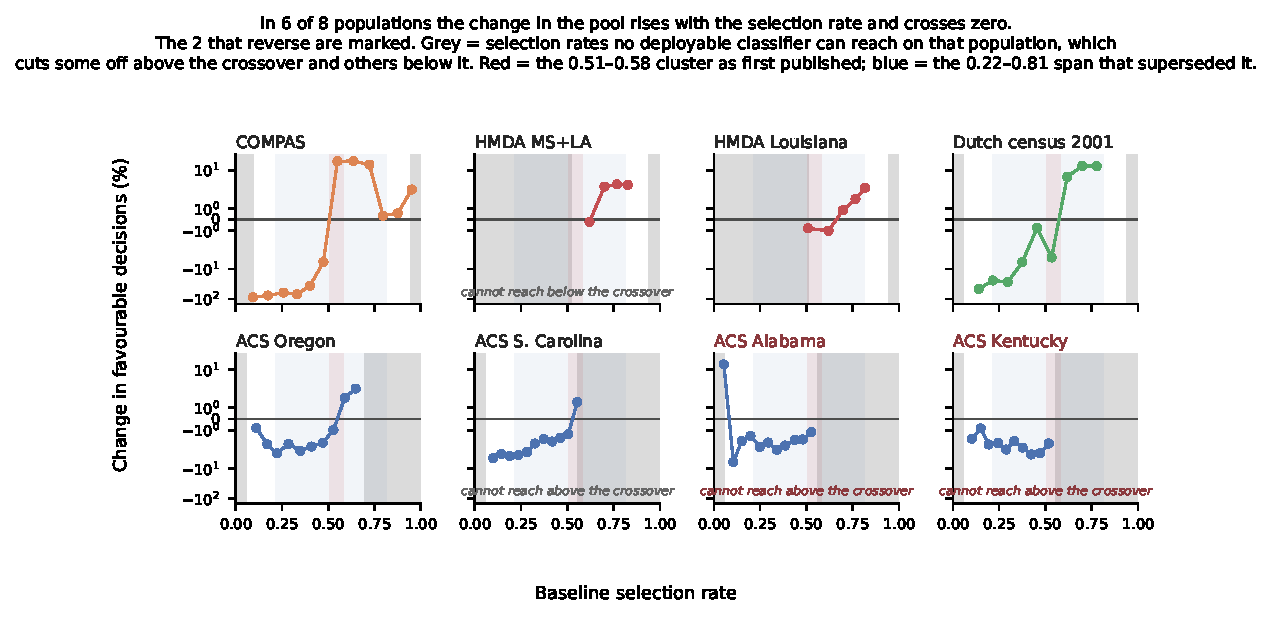
\includegraphics[width=0.84\textwidth]{fig-crossover.pdf}
\caption{Every retained arm from every densely swept population. Within a population the
change in the pool rises with the baseline selection rate and crosses zero; the two that
reverse are marked, and both are sweeps whose viable band confines them below the crossover.
Panels are deliberately \emph{not} pooled: no pooled slope survives its pre-registered bar,
so one scatter would assert a common curve the data reject. Vertical band: the point-estimate
cluster of Table~\ref{tab:crossover}, drawn as first published;
Section~\ref{sec:boundaries} gives its later history.}
\label{fig:crossover}
\end{figure*}


\subsection{A single-factor design}

ACS Income's label is ``earns more than \$50{,}000'', and that threshold is a benchmark
convention rather than a fact about the world, which makes it a knob we can turn. Moving it
on one fixed state varies the selection rate while the sampled people, instrument,
feature set and group ratio stay fixed --- though moving the label redefines the
prediction problem itself, so this is one arm of the two-routes triangulation below, not
an isolation of the rate on its own. The change in the pool rises with the
baseline selection rate at $r = +0.801$ over four arms --- too few points for formal
inference, and reported as descriptive; a partial correlation on four points has one
degree of freedom and is omitted as uninformative. The sign flip is the substantive
observation: 22 decisions are destroyed per one created at a rate of 0.03, compared with
0.75 at 0.89.

\subsection{The transition appears without being manufactured}

The same transition also appears where nothing is manipulated at all. Pooling two states
across five real loan products, home improvement at a selection rate of 0.555 levels
\emph{down} ($-1.57\%$) while refinancing at 0.871 levels \emph{up} ($+2.95\%$), with
$r = +0.803$ and Spearman $\rho = +0.900$. This means a bank running one constraint across
its loan book would take opportunities away in one product while handing them out in
another, and its fairness report would show success in both.

\subsection{It is the rate, not the difficulty of the task}
\label{sec:tworoutes-note}

\begin{figure*}[t]
\centering
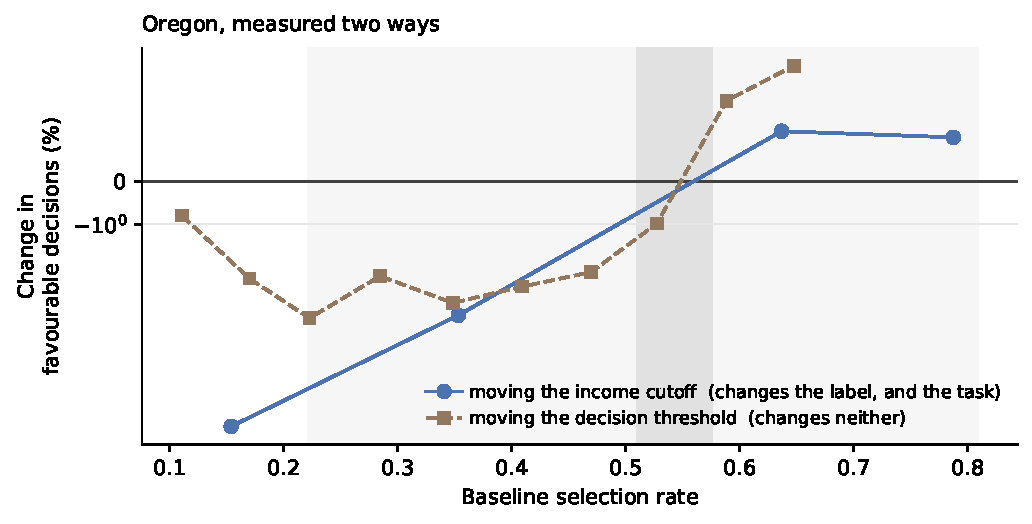
\includegraphics[width=0.86\textwidth]{fig-two-routes.pdf}
\caption{The design that separates the selection rate from the difficulty of the task. Moving
the income cutoff changes the label, and therefore how hard the problem is; moving the decision
threshold changes neither, only where the fitted model draws its line. Both routes cross zero
inside the same band. If difficulty were doing the work, the second curve would not reproduce
the first.}
\label{fig:tworoutes}
\end{figure*}


The design above moves the \emph{label}. ``Earns over \$100{,}000'' is not a rarer version of
``earns over \$20{,}000''; it is a harder problem. That design therefore cannot separate two
explanations which predict everything observed so far.

We separate them by holding the task completely fixed --- same rows, features, groups and
\emph{fitted scores} --- and moving only where the model draws its line. The relationship
reproduces, and so does the crossover's location: on Oregon the two routes give 0.362--0.653
and 0.353--0.637 (Fig.~\ref{fig:tworoutes}). \textbf{Task difficulty is not doing the work.}

With twelve points chosen from each population's viable band, the relationship holds on the
Dutch census ($+0.946$), South Carolina ($+0.905$) and COMPAS ($+0.844$). Alabama and Kentucky
return \emph{negative} values on eleven and ten arms; their viable bands top out at 0.566 and
0.561, at or below every crossover measured, so both sweeps lie almost entirely on one side of
the transition. \textbf{We therefore claim the relationship across the crossover and withdraw
any claim that it holds within the low-rate region alone.}

\subsection{Five domains, and the group-gap alternative}

\begin{table}[t]
\caption{The relationship across instruments, not pooled across them, for the reason
Fig.~\ref{fig:crossover} does not pool. This table's job is \emph{breadth} --- one population
per instrument, on whatever arms that population naturally supplies --- so the four-to-six-arm
correlations are descriptive, exactly as Section~\ref{sec:tworoutes-note} concedes for Alabama.
The dense-sweep columns carry the statistical weight where a viable band allows twelve points:
those are the same populations at $n = 12$, where the relationship is significant at
$p < 0.001$. The pre-registered alternative is refuted on the dense columns, not the sparse
ones.}
\label{tab:domains}
\centering
\scriptsize
\setlength{\tabcolsep}{2.5pt}
\begin{tabular}{@{}lllcccc@{}}
\toprule
& & & \multicolumn{2}{c}{\textbf{natural arms}} & \multicolumn{2}{c}{\textbf{dense sweep}} \\
\cmidrule(lr){4-5}\cmidrule(lr){6-7}
\textbf{Instrument} & \textbf{Domain} & \textbf{Population} & \textbf{$r$} & \textbf{n} &
\textbf{$r$} & \textbf{n} \\
\midrule
ACS Income & income & Alabama & $+0.801$ & 4 & --- & --- \\
ACS Income & income & S. Carolina & --- & --- & $+0.905$ & 12 \\
HMDA & mortgages & MS+LA pooled & $+0.858$ & 4 & --- & --- \\
COMPAS & crim. justice & race arm & $+0.870$ & 5 & $+0.844$ & 12 \\
Dutch census & occupation & sex arm & $+0.915$ & 6 & $+0.946$ & 12 \\
LSAC & legal educ. & --- & unsweepable & --- & --- & --- \\
\bottomrule
\end{tabular}
\end{table}

Fig.~\ref{fig:crossover} shows every arm, and Table~\ref{tab:domains} the summary. The
pre-registered alternative --- ``this is a property of income prediction and American mortgage
lending'', requiring $|r| < 0.30$ --- is refuted on both new instruments, and refuted on their
\emph{densely swept} arms rather than their sparse ones: COMPAS gives $+0.844$ and the Dutch
census $+0.946$ over twelve points each, both significant at $p < 0.001$. The four- and
five-arm rows are reported for breadth and carry no inferential weight on their own.

The oldest competing account is that the \emph{gap between groups} drives the direction. The
Dutch census has a gap of 0.298, roughly twice Adult's, making it the population where that
explanation should win. It gives $r = +0.915$ across all six arms, none excluded.

Because the parity-gap floor was tuned in-sample (Section~III), every row of
Table~\ref{tab:domains} was re-scored at floors 0.02/0.05/0.08/0.10: each correlation
stays between $+0.80$ and $+0.92$ with no sign change at any floor (HMDA is
floor-invariant outright; Alabama thins to two arms only at 0.10). The floor dependence
that Table~\ref{tab:sensitivity} reports for the exploratory states does not reach the
domain table.

\subsection{Robustness}

\begin{table}[t]
\caption{What each manipulation preserves}
\label{tab:robust}
\centering
\small
\begin{tabular}{@{}lll@{}}
\toprule
\textbf{Manipulation} & \textbf{Direction} & \textbf{Magnitude} \\
\midrule
Route to the rate & unchanged & differs $3\times$ \\
Tolerance, $25\times$ range & unchanged & differs $4\times$ \\
Boosted trees (5/5 pops.) & unchanged & differs $3\times$ \\
Attribute, sex $\rightarrow$ race & unchanged & --- \\
Criterion $\rightarrow$ equalized odds & weaker, unevenly & differs $8\times$ \\
Optimiser $\rightarrow$ post-proc. & \textbf{vanishes} & --- \\
\bottomrule
\end{tabular}
\end{table}

Table~\ref{tab:robust} summarises. \textbf{Within a population, and in the attribute-blind regime, the selection rate
predicts which way and orders how much. Neither transfers between populations}: the signed distance from a
population's own crossover gives $\rho$ of $+0.96$, $+0.95$ and $+0.78$ in three of four
populations, but a pooled slope reaches only $r = +0.487$ against a pre-registered $+0.70$ bar.

\section{A Constraint on One Attribute Leaves Subgroups Behind}

\begin{table}[t]
\caption{UCI Adult. Constraining sex to 0.020 leaves the worst \emph{Sex}$\times$\emph{Race}
subgroup gap at 0.178 --- nine times larger --- and moves which subgroup is worst off.}
\label{tab:intersectional}
\centering
\footnotesize
\setlength{\tabcolsep}{4pt}
\begin{tabular}{@{}lccl@{}}
\toprule
\textbf{Arm} & \textbf{Sex} & \textbf{Subgroup} & \textbf{Worst off} \\
\midrule
Unconstrained & 0.190 & 0.315 & F$\times$Black \\
Constrained on sex & \textbf{0.020} & \textbf{0.178} & M$\times$Black \\
Constrained on both & 0.016 & 0.048 & F$\times$White \\
\bottomrule
\end{tabular}
\end{table}

A constraint is imposed on the attribute someone chose to name.
Table~\ref{tab:intersectional} is the gerrymandering failure of Kearns \emph{et al.}
\cite{kearns2018} measured on Adult.

Constraining sex drives its gap from 0.190 to 0.020 --- a success by the certifying metric.
The worst \emph{Sex}$\times$\emph{Race} subgroup gap falls only from 0.315 to 0.178, which is
\textbf{nine times} the gap that was constrained. The subgroup carrying the residual also
\emph{changes}, from Female~$\times$~Black to Male~$\times$~Black, so an auditor tracking the
originally worst-off cell would see improvement while a different cell absorbed the cost.

This replicates across populations and is more severe than Adult suggests: 13.2$\times$ in
Mississippi. It is bounded, however, by how large the minority is --- the effect scales with
minority share at $r = -0.671$, and does not appear at all below a threshold. We present this
as an empirical replication of \cite{kearns2018} and \cite{maheshwari2023} with a boundary
attached, not as a new observation.

\textbf{A measurement hazard worth naming.} Roughly five subgroups per population are too small
to support any estimate. A rate with an empty denominator must return undefined rather than
zero, or an unmeasurable subgroup masquerades as a perfectly fair one --- which is the failure
this analysis is most likely to produce and hardest to notice.

\section{The Regime Boundary}
\label{sec:regime}

The last row of Table~\ref{tab:robust} looks like a failure of robustness, and for two
review rounds we read it as falling exactly on the line the theory draws: post-processing
reads the protected attribute at prediction time while the reduction does not, and that
is the distinction on which \cite{backfire2026} is built.

Running post-processing at each population's natural operating point across 17 populations
gives $r = -0.024$, compared with $+0.585$ for the reduction on the same populations. Our
pre-registered prediction --- that the rule would carry over --- failed, and its naive
alternative won outright, which is what pointed us at the regime distinction in the first
place.

\textbf{That reading was confounded, a reviewer said so, and the deconfounding test
changed it.} The contrast above moves two things at once --- attribute access \emph{and}
the optimizer family --- so ``the boundary is attribute access'' and ``the boundary is
the method'' were observationally equivalent in everything reported so far. The missing
cell was sealed with both readings' bars committed in advance (theory reading:
$|r| < 0.30$; method reading: $r \ge +0.40$; a declared dead zone between) and run:
the \emph{same} reduction, on document~43's eighteen populations, with the protected
attribute in the feature set. The relationship stands --- $\mathbf{r = +0.672}$ across
the thirteen natural arms surviving the frozen exclusions, if anything stronger than the
blind cell's $+0.585$. \textbf{The pool-direction boundary is therefore the method
family, not attribute access}: blindness is not load-bearing for the claim, the
$-0.024$ vanishing is a property of threshold re-derivation rather than of reading the
attribute, and the rule's applicability widens to attribute-aware in-processing, on
the strength of one sealed cohort.

\textbf{What survives untouched --- strengthened, in fact --- is the theory's own
group-level claim}: where the attribute is readable, the advantaged group loses and the
disadvantaged gains, always. On our post-processing populations that holds in
\textbf{18 of 18}, without exception --- and the deconfounding cell extends it: under
attribute-aware \emph{in-processing} it holds in a further \textbf{18 of 18}. The two
results separate cleanly: the theorem determines each \emph{group's} direction wherever
the attribute is readable, while the \emph{pool's} direction --- the sum the theorem
does not constrain --- remains rate-predictable under in-processing in both regimes and
unpredictable only under post-processing. That check was
post-hoc, so we repeated it as a confirmatory test on nine populations never previously
post-processed, with the bar set at all nine and committed before the runs: it holds \textbf{9
of 9}. One scoring honesty: the coin-flip tail ($0.5^9 \approx 0.002$) is the wrong null
to celebrate, because the theorem made the informed prior for this outcome close to one
--- so this row is a \emph{theory-consistency check} that the pipeline reproduces what
the theorem determines, not a forecasting success, and we count it as the former. The
regime result therefore stands at 27 of 27, nine of them run to a pre-committed bar.
Scoring is strict rather than weak: an arm counts only if the advantaged group's seed-mean
losses and the disadvantaged group's seed-mean gains are both positive, and no
minimum-magnitude guard was applied --- the theorem promises weak inequalities, so a
near-zero arm could in principle have scored either way, a rubric gap the later sealed
direction tests closed and this count predates.

\textbf{A word on what we do and do not claim against the theory.} Its Theorem 3 states
conditions over the extrema of $\zeta(x) = (\eta(x)-c)/\nu(x)$, where $\eta(x)$ is the
positive-class probability at $x$, $c$ the cost threshold, and $\nu(x)$ the group-membership
signal --- which their paper leaves without a prescribed estimator, so we estimate $\nu$
with a logistic probe predicting the protected attribute from the features. \textbf{Under
that estimator, the extrema orderings could not be certified on any of the 26 arms tested}:
the plug-in $\hat\zeta$ grows without bound where $\hat\nu$ approaches zero, and the two
regions' empirical ranges overlapped in every case --- on Adult by $[-139, 4.1]$ against
$[-39, 6662]$. This is an estimator-relative finding, not a structural one; a different
estimator, or the population quantities themselves, might behave differently. The
conditions are also \emph{sufficient, not necessary}, so none of this makes the theorem
false. It leaves it \emph{unverifiable on these populations as we could measure them},
which is a claim about operational applicability and not a refutation.

The relationship between their quantity and ours turns out to be closer than a horse race.
A \emph{relaxed} version of their ordering, replacing the unattainable extrema with
5th/95th percentiles of $\hat\zeta$, agrees with the measured direction on \textbf{24 of
26} arms, compared with 25 of 26 for the selection rate --- and, in a post-hoc comparison,
\textbf{the baseline selection rate correlates with the relaxed ordering quantity at
$r = +0.935$}, the two rules agreeing on 25 of 26 arms. That is, the number this
paper uses is not a rival of the theory's condition but a cheap proxy for it: the theory's
ordering needs the joint score-and-group distribution and an estimator nobody has
prescribed, while the selection rate needs one line of a dashboard, and the two point the
same way almost everywhere. The regime distinction itself matters most: the theory says
where prediction is possible at all, and the selection rate \emph{operationalizes} its
within-regime content --- which is something an empirical study can establish and a
population-level argument cannot.

\section{Boundaries}
\label{sec:boundaries}

\subsection{The crossover clustered, until more states were measured}

\begin{table}[t]
\caption{Crossover locations, with the existence of a crossing separated from its
location. \textbf{P(crossing)} is the share of nested rows-by-seeds resamples in which a sign
change can be bracketed at all; \textbf{crossover} is the median location \emph{conditional}
on one existing. Separating them is not pedantry: read under seeds only, the Dutch census
appeared to cross at 0.576 with a 95\% interval of 0.572--0.580 --- an apparently precise
estimate --- while under the nested bootstrap \emph{no} resample brackets a crossing, and the
published figure was a property of the six arms that produced it. An interval conditioned on
an event that may not occur cannot be read as an interval. The bracket-only rows assume a
crossing rather than estimating whether there is one, and the lending rows are point estimates
with no resampling; both are labelled as such rather than sharing a column with the nested
figures. The rates are not one economic object: survey rows are predicted-status rates over
sampled persons, lending rows are approval rates conditional on having applied, and COMPAS
inverts a risk score.}
\label{tab:crossover}
\centering
\scriptsize
\setlength{\tabcolsep}{2pt}
\begin{tabular}{@{}llccl@{}}
\toprule
\textbf{Population} & \textbf{Domain} & \textbf{P(crossing)} &
\textbf{Crossover} & \textbf{Uncertainty} \\
 & & & \textbf{\emph{given} one} & \\
\midrule
\multicolumn{5}{@{}l}{\emph{Nested rows-by-seeds bootstrap, 1{,}000 pairs}} \\
COMPAS & crim. justice & 100\% & 0.457 & 0.433--0.539 \\
S. Carolina & income & 97\% & 0.525 & 0.454--0.537 \\
Oregon & income & 99\% & 0.532 & 0.514--0.604 \\
Dutch census & occupation & \textbf{0\%} & --- & none crosses \\
\midrule
\multicolumn{5}{@{}l}{\emph{Bracket only --- crossing assumed, not estimated}} \\
Florida & income & --- & \textbf{0.284} & 0.259--0.309 \\
Ohio & income & --- & 0.556 & 0.528--0.585 \\
Pennsylvania & income & --- & \textbf{0.652} & 0.624--0.681 \\
\midrule
\multicolumn{5}{@{}l}{\emph{Lending --- one market, three overlapping estimates}} \\
HMDA pooled & mortgages & --- & 0.660 & point only \\
HMDA Louisiana & mortgages & --- & 0.659 & point only \\
HMDA refinance & mortgages & --- & 0.758 & point only \\
\bottomrule
\end{tabular}
\end{table}

Table~\ref{tab:crossover} tells the honest history in three blocks. The first four
populations, across three domains and two countries, have overlapping intervals, and
carrying those intervals gave a cluster spanning roughly 0.43--0.58. Because the
table's original intervals resample seeds only --- an anti-conservative choice the
Setup section concedes --- the four located rows were re-run under a nested
rows-by-seeds bootstrap (five refitted seeds $\times$ 200 row resamples of the test
split, arms rebuilt per seed at fixed target rates). Three survive: COMPAS, South
Carolina and Oregon's published locations sit inside their nested 95\% intervals
(medians 0.457, 0.525, 0.532), with a crossing bracketed in over 97\% of resamples.
\textbf{The Dutch row does not}: under the denser view its mid-band signs interleave
and no (seed, resample) pair brackets a crossing at all, so its 0.576 is downgraded to
a property of the six arms that produced it, consistent with the non-monotone verdict
the audit itself returns on that population. A design-weighted re-reading of the ACS
rows (models unchanged, evaluation under PWGTP) shifts every bracket down by
0.03--0.08 while Florida and Pennsylvania remain the outliers --- the located span
\emph{widens} weighted --- so the ordering is weighting-robust and the numeric
locations belong to the unweighted convention the Setup declares. A sealed sweep campaign
across ten further states was then run to test what predicts the location, and the three
crossovers it located break the cluster: Ohio lands inside it, while \textbf{Florida sits at
0.284 and Pennsylvania at 0.652}, both with tight brackets and every guard passed, on the
same instrument the cluster was built from. Located crossovers now span \textbf{0.28 to
0.65}, which means the location is population-specific, often but not reliably near the
middle. The same campaign found that a third of the large states have no crossover to
locate at all: Texas, New York and Illinois sweep U-shaped, with the pool change positive
at both window edges and negative between, while New Jersey and Virginia level \emph{up}
across their entire windows. The monotone within-population picture, which held on every
population swept before, is therefore itself population-dependent.

The natural-arm route has since been run on \textbf{every market in the country}: all fifty
states, both protected attributes. On race arms the direction rule holds wherever the audit
will accept the arm at all --- 25 of 31 clearing the parity floor, and \textbf{12 of 12}
clearing both that floor and the one-point magnitude guard, at rates 0.823--0.898 where the
rule predicts extension. That supersedes the seven-of-eight this section previously rested
on, which came from a single pooled market.

\textbf{The sex arms are refused, and the refusal is the finding.} Not one of the twenty-six
markets carrying a sex arm clears the audit's 0.05 disparity floor: the median baseline gap
is 0.013 against the race arms' 0.079, the median pool change is 0.02\%, and no arm moves by
a full point. US mortgage approval carries a substantial race gap and essentially no
measurable sex gap, so there is nothing for a parity constraint to close and the sign of what
movement there is carries no information. This is the same refusal Brazil produced in the
third cohort, on a different continent and a different instrument, and it is a better
argument for the disparity floor than any reasoning about it.

A mechanism for those failures has since turned up. All three home-improvement sweeps run
on fresh markets return the same non-monotone \mbox{$+\,\ldots\,-\,\ldots\,+$} shape, so a
bracketing step that assumes one rising crossing cannot read them --- which is what a sweep
scored 2 of 4, and later 2 of 6, was failing to do.

Every lending estimate sits above every non-lending one, but those come from a \emph{single}
market measured three overlapping ways, so ``lending is different'' remains a hypothesis
--- and selection into that market's sample is the leading alternative reading: an HMDA
approval rate conditions on who applied, which the survey rates do not.

\subsection{The shape boundary, taken cross-task}
\label{sec:crosstask}

A twelfth sealed test asked whether the curve-family boundary of the shape seals --- LOW
below a label base rate of 0.365, HIGH at or above --- survives a change of
\emph{question}. Six race arms of two folktables tasks this project had never run
(employment in three states, public-coverage receipt in three) were sealed with
seed-0-fixed thresholds, calls on both sides of the boundary, and the seal's commit
externally timestamped before any arm existed. \textbf{It scored 0 of 4} (two sweeps
returned too few surviving arms to classify), against a bar of scored$-$1, the constant
not beaten. What that settles must be stated carefully, because every scored call was
wrong \emph{in the same way}: a perfect inversion is transferred structure with a
flipped sign, not the absence of structure, and with two tasks sharing persons this
design cannot separate ``the boundary is income-specific'' from ``the boundary's sign
depends on the task family'' or from a parameterization we have not identified. Two
artifacts are ruled out: the family call is computed from pool-change signs, which are
invariant to the group declaration, and the labels are folktables' own, so neither of
the convention errors our checks guard against can produce this pattern. Recorded
beside the failure, without a registered bar: all six populations' natural arms moved
\emph{down}, at rates 0.31--0.47 --- what the direction rule expects below the
crossover, though a constant predicting ``down'' matches it equally, so it is a
consistency observation and no more. The boundary's remaining live test is the IPUMS
cohort's S3, on income tasks, real-anchored --- the only domain where it has ever
called anything correctly.

\textbf{The transported prior carries a dead band, and the procedure did not previously
say so.} Pooling every arm from all four sealed direction cohorts and scoring each against
its own cohort's crossover gives a calibration: the rule is correct on 19 of 19 arms more
than 0.30 from the crossover, 23 of 27 between 0.15 and 0.30, 5 of 6 between 0.05 and 0.15
--- and \textbf{1 of 6 within 0.05}. The last figure is not significant on six arms, but its
arms have since been swept, and the answer is not the one we first proposed. Maryland's own
crossover sits at 0.15--0.29, so its natural rate of 0.508 is far above it, the rule read
against \emph{its own} crossover says up, and it went up: that miss is the transported
prior's want of resolution, exactly as one would expect of a fixed value when located
crossovers span 0.28 to 0.65. \textbf{The other five are not misplaced crossovers at all.}
Their sweeps have no single rising sign change --- four are non-monotone and Missouri is
outright inverted --- so no directional rule applies to them, and
Algorithm~\ref{alg:locate} returns \textsc{non-monotone} on every one. The sixth is the
control: it is the arm the rule got \emph{right}, its landscape is non-monotone too, and so
its correctness was luck rather than skill. \textbf{What the dead band exposes is therefore
not a failure of the rule but a blind spot of the prior}: detecting a non-monotone landscape
requires the sweep that transporting a prior exists to avoid, so a team reading 0.54 off a
dashboard cannot know the rule does not apply to them. The procedure was never exposed here;
only the prior was.

\textbf{We therefore treat a crossover near 0.54 as an empirical prior with a measured
failure rate, not a constant.} It predicted 9 of 10 sealed populations in advance
(Section~\ref{sec:resealed}); scored post-hoc on the campaign's ten natural arms it manages
5 of 10, and every miss agrees with its own state's sweep --- Florida's natural arm turns up
at a rate of 0.288, and Florida's located crossover is 0.284. That agreement carries the
same caveat as the audit's consistency count: the natural arm is part of the sweep that
located the crossover, so miss-agreement is a post-hoc, partially circular check, not
independent validation. The within-population
relationship survives where the landscape is monotone; the fixed prior transfers to some
populations and not others, and nothing in this work yet says which in advance.

The residual question --- what predicts the location --- was given a sealed test with two
candidate predictors, a $\rho \geq 0.70$ bar and a floor of six new locations. It returned
\textsc{underpowered}: three located, so neither candidate is judged. The earlier screen's
two correlations ($+0.724$, $+0.865$, collinear at $+0.947$ over four populations) remain a
hypothesis, and any future test must first handle landscapes with no crossover at all.

\subsection{The procedure is unusable on very generous tasks}

Varying the selection rate by moving a threshold works by \emph{degrading} the classifier. On a
task where most people already qualify, reaching a low selection rate requires a model that
refuses qualified people, and past a point that model is worse than a constant. Defining the
\emph{viable band} as the range of selection rates reachable by a classifier still beating
$\max(p, 1-p)$: Dutch spans 0.895, COMPAS 0.859, typical ACS $\approx 0.51$, and LSAC only
\textbf{0.056}. On LSAC, where 89\% pass the bar, no choice of thresholds produces a usable
sweep. This is computable before running anything.

When the viable band forbids a sweep, the crossover can still be located by comparing natural
sub-populations --- which is how the mortgage crossover was first found.

\subsection{A sealed prediction, and what it cost}
\label{sec:sealed}

\begin{table}[t]
\caption{Sensitivity to the parity-gap exclusion. Correlation per population as the
threshold is loosened.}
\label{tab:sensitivity}
\centering
\footnotesize
\setlength{\tabcolsep}{5pt}
\begin{tabular}{@{}lcccc@{}}
\toprule
\textbf{Population} & \textbf{0.01} & \textbf{0.02} & \textbf{0.05} & \textbf{0.10} \\
\midrule
Dutch census & $+0.851$ & $+0.908$ & $+0.946$ & $+0.938$ \\
COMPAS & $+0.844$ & $+0.844$ & $+0.844$ & $+0.871$ \\
S. Carolina & $+0.012$ & $+0.012$ & $+0.905$ & $+0.849$ \\
Oregon & $+0.095$ & $+0.095$ & $+0.664$ & --- \\
Alabama & $-0.368$ & $-0.368$ & $-0.368$ & $+0.296$ \\
Kentucky & $-0.590$ & $-0.590$ & $-0.654$ & --- \\
\bottomrule
\end{tabular}
\end{table}

Every result above is a correlation computed after the arms were run, which is the weakest
support for a claim of the form \emph{you can know in advance}. We therefore ran the strongest
format available: nine populations whose direction had never been measured, with the rule, the
populations and the pass mark committed before any of them existed. Eight enter the sealed
score; the ninth, Taiwan, was sealed alongside them but registered as reported separately,
because a single non-Western population can carry no claim on its own (it was predicted
correctly: rate 0.885, observed $+0.68\%$).

\textbf{It failed. Four of eight, against a bar of seven, not beating a constant}
(Table~\ref{tab:sealed}).

\begin{table}[t]
\caption{The sealed prediction. Populations never previously measured; predictions committed
before the runs.}
\label{tab:sealed}
\centering
\footnotesize
\setlength{\tabcolsep}{4pt}
\begin{tabular}{@{}lrrcc@{}}
\toprule
\textbf{Population} & \textbf{Rate} & \textbf{$\Delta$pool} & \textbf{Pred.} & \textbf{Actual} \\
\midrule
MO, \$100k & 0.026 & $-16.48\%$ & up & \textbf{down} \\
AZ, \$100k & 0.037 & $-23.34\%$ & up & \textbf{down} \\
IN, \$70k & 0.081 & $-23.32\%$ & up & \textbf{down} \\
TN, \$50k & 0.255 & $-1.68\%$ & down & down \\
MD, \$50k & 0.508 & $+0.78\%$ & down & \textbf{up} \\
MI, \$30k & 0.612 & $+0.85\%$ & up & up \\
NC, \$20k & 0.789 & $+0.16\%$ & up & up \\
GA, \$10k & 0.905 & $+0.30\%$ & up & up \\
\midrule
Taiwan 2005 & 0.885 & $+0.68\%$ & up & up \\
\bottomrule
\end{tabular}
\end{table}

\textbf{What failed is a refinement, not the rule.} Table~\ref{tab:sensitivity} shows the
exclusion threshold doing real work: South Carolina moves from $+0.905$ to $+0.012$ when it is
loosened. Investigating that, we found the newly admitted arms are not noise --- at twenty
seeds they are consistently \emph{positive}, $+8.73$, $+6.85$, $+9.09$, six standard errors
from zero --- and concluded the relationship turns back up below a selection rate of 0.10. The
sealed rule carried that refinement.

All three held-out low-rate arms came out strongly \emph{negative}. Scoring the same eight arms
under the simpler rule we held before the refinement --- down below the crossover, up above it
--- gives \textbf{seven of eight}, its only miss being Maryland at 0.508, within 0.032 of the
crossover on an effect of $+0.78\%$. That seven is post-hoc and we do not claim it; what was
sealed scored four.

\textbf{The refinement was route-specific.} Its arms reach a rate near 0.05 by thresholding one
fixed score vector; the sealed arms reach it with a genuinely rarer label. At that rate the two
disagree completely, $+8.73$, $+6.85$, $+9.09$ against $-16.48$, $-23.34$, $-23.32$. So
Section~\ref{sec:tworoutes-note} qualifies: the two routes agree through the middle of the range
and diverge at the bottom, and the accuracy rule does not catch the divergent arms --- they
clear the trivial-predictor bar and remain artifacts.

A refinement drawn from four in-sample populations, internally consistent and backed by a
twenty-seed replication, made the prediction worse than the rule it replaced and no better than
a constant. Nothing in the in-sample data could have shown that.

\subsection{The rule re-sealed, and it holds}
\label{sec:resealed}

\begin{table}[t]
\caption{The re-sealed prediction: the unrefined rule --- down below 0.54, up at or above ---
committed before ten never-measured states ran. Bar: 9 of 10 \emph{and} beat the best
constant.}
\label{tab:resealed}
\centering
\footnotesize
\setlength{\tabcolsep}{4pt}
\begin{tabular}{@{}lrrcc@{}}
\toprule
\textbf{Population} & \textbf{Rate} & \textbf{$\Delta$pool} & \textbf{Pred.} & \textbf{Actual} \\
\midrule
NE, \$100k & 0.014 & $-6.35\%$ & down & down \\
AR, \$50k & 0.195 & $-2.55\%$ & down & down \\
OK, \$50k & 0.220 & $-12.78\%$ & down & down \\
WA, \$70k & 0.233 & $-5.52\%$ & down & down \\
NV, \$50k & 0.297 & $-1.57\%$ & down & down \\
MN, \$30k & 0.699 & $-0.04\%$ & up & \textbf{down} \\
CO, \$30k & 0.701 & $+0.63\%$ & up & up \\
KS, \$20k & 0.767 & $+0.58\%$ & up & up \\
WI, \$20k & 0.814 & $+0.69\%$ & up & up \\
IA, \$10k & 0.896 & $+0.04\%$ & up & up \\
\bottomrule
\end{tabular}
\end{table}

After that failure, the only move that could settle anything was to seal the \emph{unrefined}
rule --- down below 0.54, up at or above, with no low-rate clause --- against populations
with no measurement history of any kind. We used ten ACS states this project had never
touched, one arm per state so that the arm count is the population count by construction,
with income cutoffs assigned to spread the expected rates across both sides of the crossover
so that no constant could mimic the rule. The 0.54 prior itself predates the test: it is the
mid-point of the non-lending cluster, fixed from four populations that include none of the
ten. One of those four anchors --- the Dutch census --- was later downgraded by the nested
bootstrap (Section~\ref{sec:boundaries}); recomputed from the three surviving locations
the mid-point is 0.53, and no call in either sealed cohort, nor in the post-hoc campaign
scoring, changes under that shift --- the nearest arm to the boundary on any cohort sits at
0.508. The committed prior stands as sealed; its provenance is simply thinner than first
stated. The bar was committed with the populations before any arm ran: at least 9 of 10,
\emph{and} strictly beating the best constant.

\textbf{It holds: 9 of 10, best constant 6} (Table~\ref{tab:resealed}). Two statistics,
because they answer different questions and the weaker one is the honest headline. The
exact binomial tail --- a guesser at the best constant's rate ($p = 0.6$) reaches 9 or
more of 10 with probability $\approx 0.046$ --- answers whether an independent guesser
could do this. The \emph{paired} comparison against the best constant on the same ten
resolved arms is stricter: rule and constant disagree only on the five arms the rule
called \emph{up}, the rule wins four of those five, and the one-sided sign test on the
discordant calls gives $p \approx 0.19$. And this is the second sealed attempt at a
direction rule after the first failed, so even the binomial tail carries a sequential
correction of roughly a factor of two --- putting the corrected tail near 0.09, across
the conventional line: suggestive, not significant, under the sequential accounting. The
pass is evidence, not proof, and the paired test is why we claim no more. A further limit of
the cohort's own design must be stated: every arm reaches its rate by the label route, and
the achieved rates leave the interior of $(0.30, 0.70)$ unsampled --- the nearest arms
sit at its very edges (0.297, 0.699, 0.701) --- so this pass cannot discriminate the
selection rate from label rarity as the operative variable, nor the value 0.54 from any
prior in that interval --- a rule reading only the income cutoff scores identically here.
What the pass establishes is that a mid-band rule predicts direction on unseen
ACS-instrument populations; the adequately powered third cohort must therefore be
off-instrument, concentrate rates near the crossover, mix both routes, and score against
the cutoff-only and 0.5-prior nulls. That cohort has since run, two-stage sealed and
externally anchored, on the Brazilian and Mexican censuses --- and returned
\textsc{underpowered} on every component: Brazil's baseline sex gaps at the sealed
labels (0.005--0.039) fall below the 0.05 disparity floor, so the audit's own first
gate refused most of the cohort, off-instrument and off-continent, exactly as it
refused the diabetes screen. On the seven surviving in-band arms, recorded without a
verdict, the rule scores 5 of 7 and the cutoff-only null 6 of 7. The confound is
therefore resolved by the follow-on cohort rather than left open. A race-arm cohort,
screened first under the gate that failure created (Brazilian White vs Black-or-Brown
gaps of 0.13--0.17), ran powered: the cutoff-only null scored \textbf{5 of 10}
against the rate rules' 8--9 on mixed-route arms where the label's rarity was held
constant --- \textbf{it is the rate}. Its denominator must be read as what it is: those
ten arms are \emph{two} person-samples, Brazil 2000 and Brazil 2010, contributing five
arms each, four of which are operating points on the same people. The comparison is
within-population by construction and the effects are large --- to $-47\%$ --- but ten
arms from two samples is not ten independent tests, and the confound is broken on two
populations rather than on ten. Two clusters admit no usable bootstrap --- there are three
distinct resamples --- and leaving either population out drops the rate rule from 8 of 10
to 60\%. The result is real and its effects are large; its \emph{replication} rests on two
person-samples and should be read that way. The sealed S1 nonetheless FAILS by its own
letter, because a 0.50 prior edged the 0.54 prior 9 to 8: in-band, on Brazil, the
specific value holds no privilege, and Brazil's own crossovers (0.481--0.539 and
0.539--0.598) straddle both priors --- the population-specific picture this paper has
claimed throughout. The within-population component holds sealed, $\rho = 1.0$ and
$0.9$, classic crossings, effects to $-47\%$. Three crossovers are now located
outside the United States: the two Brazilian brackets and Mexico 2015 at
0.423--0.483, below the US survey cluster. The prediction used
the baseline selection rate and the fixed 0.54 prior alone --- no sweep, no per-population
characterisation. Below 0.10, where the refuted refinement said up, Nebraska at 0.014 moved
down by 6.35\%, as the unrefined rule predicts.

The miss is scored by the criterion sealed with it, and it is \emph{not} excused as a boundary
call: Minnesota sits at 0.699, far from the crossover, so under the registered rubric it
counts against the rule itself. What can be said post-hoc is that its effect is the smallest
in the set by an order of magnitude and flips sign across seeds (mean $-0.04\%$) --- a rule
predicting a sign has nothing to grip on an arm whose true value may not have one, while
Colorado, 0.002 away in rate, moved $+0.63\%$ and was called correctly. The registered rubric
did not anticipate near-zero magnitudes away from the boundary; a future seal should state a
minimum-magnitude guard in advance, and this one is charged the miss for not having done so.

A third cohort, built after this one to give the paired statistic more discordant arms,
failed for a reason worth stating here: a pre-committed magnitude guard removed ten of its
twenty-four arms, and it removed them near the crossover, because effect size grows with
distance from it ($r = +0.648$). Four discordant arms survived, the rule won all four, and
four of four is $p = 0.0625$ --- the bar was unreachable. Both of that cohort's named nulls,
the cutoff-only reading and a 0.50 prior, then scored identically to the rule on every
scored arm, with \emph{zero} discordant arms between them: like the cohort below, it
separates neither the rate from the cutoff nor 0.54 from 0.50. The guard and the
discordance a paired test needs are anti-correlated by construction, so this weakness does
not yield to a larger balanced cohort.

A seed-level accounting sharpens the lesson: 16 of the 19 sealed arms (both cohorts) are
unanimous in sign across their five seeds, and the three that split are exactly the
near-zero effects. Minnesota, the miss, splits 3 of 5 --- and Iowa, at $+0.04\%$,
splits 3 of 5 identically \emph{and scored correct}: two statistically indistinguishable
arms, one counted for the rule and one against it, which is what scoring near-zero
magnitudes means and why Algorithm~1 now refuses them as \textsc{indeterminate}.

One post-hoc robustness check, run because the exclusion rules were tuned in-sample
(Section~III) and the sealed cohorts are where their choice must not matter: the sealed
scoring used no parity-gap exclusion by design, and re-scoring under the audit's own
frozen 0.05 floor retains eight of the ten arms at 7 correct against a best constant of
5 --- the margin survives. The two arms the floor drops (Iowa and Nebraska, baseline gaps
0.016 and 0.017 at their extreme rates) are arms Algorithm~1 itself would refuse as
having too little baseline disparity to audit, which is worth knowing: the cohort's
extreme-rate coverage came partly from arms the deployable procedure would screen out.

\subsection{Small populations}

Below roughly 2{,}500 test subjects the method's own randomness exceeds the entire effect of
the constraint. This is a specific instance of predictive multiplicity
\cite{black2022,long2023} --- and Long \emph{et al.} \cite{long2023} show fairness
interventions themselves exacerbate it ---
models with equivalent aggregate performance disagreeing substantially on individuals --- and
we position it as a caution supported by that literature rather than as a novel finding. COMPAS has 1{,}584 and flips sign between seeds on two of four arms; LSAC has
6{,}240 and flips on none. COMPAS carries direction here and never magnitude.

\subsection{How the withdrawal is implemented: a lottery}
\label{sec:lottery}

The reduction returns a randomized mixture by design \cite{agarwal2018}, and each person's
approval probability under that mixture shows which solution the optimiser found. On
threshold-sweep arms deep in the score distribution's tail, two qualitatively different
solutions appear. Where the constraint \emph{lifts}, the mixture behaves like an informed
adjustment: probability is granted below the threshold, rising with the person's score,
with the disadvantaged group favoured within each score band. Where it \emph{cuts}, the
mixture is a lottery: nobody below the threshold receives any probability at all, and
every predicted positive of both groups is kept with one flat probability --- 0.65 on the
Dutch census arm, 0.135 on COMPAS, where a person's keep probability is constant in their
own score (the correlation is degenerate: score carries no information about who is kept). The gap closes because discarding a fixed
fraction of everyone's approvals at random shrinks it multiplicatively; the certificate
reports the same success either way. A single quantity --- the mean probability granted
just below the threshold --- separates the two behaviours on all nine deep-tail arms
tested, including a matched pair that agrees on every aggregate we can compute and moves
in opposite directions. Direct inspection of the fitted mixtures confirms the structure
member by member: on the cut arms the dominant-weight members grant almost nothing
(COMPAS: weights 0.86--0.88 on members whose positive rate is at most $10^{-4}$; LSAC:
0.876 on a member at $3 \times 10^{-4}$), while every lift arm's members all grant at
graded rates --- the ``one member grants nothing'' form is observed, not inferred.

Because the nine arms above sit in the region our own limitations call unreliable, the
same probe was run as a control at the \emph{natural} operating point of nine
populations spanning both directions and both instruments --- Adult, three cutting and
three extending survey populations, and the two lending markets, since the
adverse-action implication below is a lending argument. \textbf{The lottery does not
appear at any of them}: every natural-point
mixture is graded, granting probability below the boundary (means 0.17--0.63 against
0.00--0.07 on the deep cut arms) with keep probability rising in the person's own score
(correlations $+0.36$ to $+0.73$ against $\approx 0$), even on Adult, whose constraint
removes a fifth of the pool. The signature is therefore a property of constraints pushed
to severe operating points, not of withdrawal as such --- which narrows the hazard and
sharpens the audit: a flat keep probability in one's own fitted mixture is not the
expected cost of parity but a flag that the optimiser has stopped using the scores, and
the quantity that detects it is computable from any fitted mitigation.

Three delineations keep this claim its right size. In the \emph{attribute-aware} setting,
the optimal randomized fair classifier is characterized as randomizing at group-specific
decision boundaries \cite{agarwal2022}; the attribute-blind analogue is not characterized,
and a flat keep-probability is what a two-member blind mixture produces when one member
grants nothing --- which is the observed structure here; two distinct-threshold members
would instead produce a rising step --- so the lottery differs in form from the
aware-regime optimum. Whether it is
suboptimal \emph{within} the blind constrained class was an open computation; we ran
it. Searching the minimal richer class --- two-threshold blind mixtures, with the
parity weight in closed form and the threshold grid extended into the 0.9975 score
quantile to rule out a grid-edge artifact, with the pool matched to $\pm 0.005$ and the
parity gap capped at the lottery's own --- \textbf{the feasible set is empty on all
ten seed-arm pairs}: no score-informed blind mixture \emph{of that two-threshold form}
attains the lottery's parity gap and pool size at either signature arm. Within the
class searched, then, the lottery is not an optimiser failure; richer blind classes
(more thresholds, mixtures over refits) remain unsearched, so the claim is
family-relative and stated as such. What it licenses is narrower and still useful:
the obvious repair a reviewer would propose does not exist, which is exactly why the
honest charge is the missing announcement, not the randomization. The known
arbitrariness of fair models is \emph{across} retrained models \cite{long2023}; this is
deliberate randomization inside one fitted model. And randomness itself has been advocated
as a fairness device \cite{grgic2017}, and the philosophical literature holds that a
lottery among relevantly equal claims can be exactly what fairness requires
\cite{broome1990,stone2011} --- so the charge here is deliberately narrower than
``a lottery occurred'': it is that a lottery occurred \emph{unannounced}, under a
certificate indistinguishable from an informed adjustment, in settings where
individualized reasons are owed. Accepted allocation lotteries are public about being
lotteries; this one is certified as fairness. The standard derandomization remedy \cite{cotter2019} applied
to a flat lottery amounts to re-choosing a threshold, which undoes the parity the lottery
bought; for an auditor, the flat-probability signature itself is the usable part, and it
is computable from any fitted mitigation.

\section{The Audit: Give, Take, or Refuse}
\label{sec:procedure}

Algorithm~\ref{alg:locate} states the procedure. Three of its steps are worth drawing out,
because each is a place where a plausible-looking run returns a meaningless answer.

\textbf{It can refuse.} Lines 6--8 compute the viable band and exit before any constraint is
fitted, if no threshold reaches a low selection rate with a model still beating the trivial
predictor. On LSAC that band is too narrow to sweep (Section~\ref{sec:boundaries}) and the procedure
declines, rather than returning arms that would be discarded later.

\textbf{It can return \textsc{void}.} Line 16 requires enough arms to survive the guards
and the pool to have moved at all. A
correlation computed over arms that barely move is fitted to noise: Connecticut returns
$r=-0.924$ on a spread of a tenth of a percentage point, and without this test that number
reads as a refutation of the whole finding.

\textbf{It can return \textsc{non-monotone}, and on current data it often will.} Lines
20--22 exist because the assumption behind bracketing --- one rising sign change --- is
itself population-dependent: among the ten largest states we swept, three are U-shaped
and the 2022 vintages at nominal labels invert, so a bracket step that assumed
monotonicity would return a confident wrong direction precisely there. A
\textsc{non-monotone} verdict means the directional rule does not apply to this system,
which is a first-class answer, not a failure of the audit. A sweep whose retained arms
all share one sign is the opposite case and returns that direction (line 24): the
constraint moves the pool the same way across the whole viable band, which is what
``levels up throughout'' means operationally. Two cautions the earlier version of this
algorithm kept in prose are now steps: arms below a selection rate of $0.10$ are marked
\emph{advisory} and excluded from the shape call (line 14), because below that boundary
the two routes to a rate give opposite signs (Section~\ref{sec:boundaries}) and the
accuracy guard does not catch it; and every fitted arm is probed for the flat
keep-probability signature (line 19), because a lottery under the certificate is a
finding the direction verdict alone would hide. The probe's decision rule, stated so it
can be implemented: flag an arm whose mean granted probability just below the boundary
is under 0.10 while the keep-probability's correlation with the score above it is
$\approx 0$ --- the observed separation is wide (0.00--0.07 against 0.17--0.43, and
$\approx 0$ against $+0.37$ to $+0.73$). Provenance of the remaining guards, since
tuned constants are where exclusions hide: the 0.40 band span, the 2-point void guard,
the 12-threshold grid and the 0.10 advisory boundary all come from the exploratory
phase, like the two exclusion rules whose provenance Section~III discloses; all are
frozen verbatim in the third cohort's committed protocol, and ``within seed noise'' in
line 28 is the 1.0-point magnitude guard that protocol states.

\textbf{It can return \textsc{indeterminate}.} Lines 28--29 refuse a sign call when the
deployed rate sits inside the located bracket, or when the nearest arms' effects are
within seed noise --- precisely the two conditions under which this project's own record
shows a sign call has nothing to grip: Maryland's miss sat at the cluster's edge
(Section~\ref{sec:sealed}), and Minnesota's was an effect of $-0.04\%$ that flips sign
across seeds. The registered
rubric of the re-seal did not have this verdict and was charged a miss for it; the
algorithm inherits the lesson.

\textbf{The magnitude guard is measured, not assumed.} Line 28's refusal rests on the
claim that a near-zero effect has no sign to predict. Two sealed cohorts run after this
algorithm was written put a number on it: across their forty arms the rule is correct on
\textbf{21 of 22} arms whose effect exceeds one point and on \textbf{11 of 18} below it ---
95\% against 61\%, which is a coin flip. Those arms span 19 and 15 disjoint person-samples,
and clustering on the sample rather than the arm leaves the split intact: 85--100\% above
the threshold against 37--82\% below, intervals that barely meet. The threshold is doing
what it claims.

\textbf{It returns a sign, never a size.} The distance from the crossover \emph{orders} the
effect within a population, so a team can rank its own segments; but no slope transfers between
populations, so lines 32 and 34 return a direction and stop there.

\textbf{What it is for, and what it is not.} The audit applies where the pool of
favourable decisions can actually change size. Where the allocation is
capacity-pinned --- a fixed number of seats, beds, or slots --- the total is constant
by construction, the directional quantity this paper measures cannot arise, and the
audit is out of scope from line~0; this is the fixed-resource regime of
\cite{goethals2024}, and clinical triage and admission commonly live there. No
natural operating point below 0.13 has been probed in this record, so deployed rates
below that carry an untested-region caution on top of every verdict.

\textbf{What it needs, and what it costs.} The audit requires a held-out sample carrying
the protected attribute: audit-time access to $a$, which is legally and practically
distinct from decision-time use and is the regime bias-testing provisions contemplate
(Section~\ref{sec:scope}) --- in US credit, the self-test privilege of Regulation~B
(12~CFR~\S1002.15) exists for exactly this, though it is conditional: the privilege
attaches to a lender's own voluntary self-test and expects appropriate corrective
action, and an analysis of public HMDA records, like this paper's, is not itself a
privileged self-test. It fits the constraint $12 \times \mathrm{seeds}$ times; with five seeds
and the linear learners used here, one fit takes 2--10 seconds at $15$k--$69$k training
rows (measured on a laptop CPU), so a full audit is minutes per population, and its cost
scales linearly in the base learner's own fit time since each reduction call is a
sequence of learner refits. A cheap pre-screen exists: the relaxed-$\zeta$ ordering of
Section~\ref{sec:regime} needs no constraint fits and correlates with the predictor at
$r=+0.935$.

\textbf{What it actually returns, totalled.} Run over the 52 population-label pairs whose
stored sweeps resolve to a dataset spec --- fourteen further IPUMS sweeps are stored but
unmapped, and are excluded rather than guessed at --- the distribution
is: 29 directional verdicts (20 \textsc{withdrawal}, 9 \textsc{extension}), 8
\textsc{non-monotone}, 13 \textsc{void}, one refusal at the noise floor (COMPAS), and
one bracket with no natural arm to read against. Every one of the 29 directional
verdicts matches what the fitted constraint did at that population's natural operating
point --- a consistency check on the audit's reading of its own sweep, not independent
validation, since the natural arm is part of the curve being read. That distribution is computed over the sweeps this project happened to accumulate, which
were never randomly chosen, so it answers a question about this project rather than about
populations. A survey with a pre-committed frame answers the latter.

\textbf{The frame, since ``at random'' means nothing without one.} Every combination of the
fifty US states, the 2014, 2018 and 2019 ACS vintages, and the two protected attributes, with
the income cutoff held at \$50{,}000 --- 300 population-label pairs. The 2022 vintage is
excluded because its inversion is a diagnosed nominal-label artifact, and including it would
conflate a label problem with a landscape property. Fifty pairs were drawn uniformly at
random under a fixed seed, and the frame, the seed, the draw and the exclusion were all
committed to version control before any arm ran; the drawn list is in the repository. The
draw came out balanced without being forced: 25 of each attribute, and 14, 14 and 22 across
the three vintages. The fifty pairs span \textbf{48 disjoint person-samples}, two state-years
having been drawn under both attributes.

The result: \textbf{78\% admit a directional rule and 22\% do not}, of which 64\% are
classic single-crossing landscapes. Resampling \emph{populations} rather than draws puts the
directional share at 66--89\%, and leaving each population out in turn never moves it below
77\%. The convenience sample was mildly optimistic --- it implied 15\% non-monotone --- and
the larger number is the one to quote. The refusals are not
silences. A \textsc{void} arm is one whose pool change spans under two points across the
entire viable band --- median 1.47 --- which tells a deployer that the direction question is
\emph{moot} on their system, not that it is unanswerable; a \textsc{non-monotone} verdict
says the rule does not apply here, which is a finding about the system; and the noise-floor
refusal says the population is too small to audit at all. Counted that way, 48 of the 52
return something a team can act on and four return nothing --- three sweeps too thin to read
and one bracket with no natural arm. The honest summary: the audit gives a \emph{direction}
a little under six times in ten, tells a team the question is moot or the rule inapplicable
in most of the remainder, and is silent on four of fifty-two. Finally, an ex-ante verdict earns trust only if checked:
whatever the verdict, including refusals, the deployed system's measured pool change and
who-pays decomposition (Section~\ref{sec:whopays}) should be reported after the fact ---
the verdict is falsifiable at deployment, and Section~\ref{sec:discussion} makes this a
requirement rather than advice.

\textbf{The direction survives the extraction a deployer must apply.} Every direction
result above is measured on the randomized mixture, but a lender under
adverse-action-notice duties deploys a \emph{deterministic} model, so we tested the
extraction directly: thresholding the mixture's per-person probability at $0.5$ on the
natural arms of ten populations spanning both directions. The extracted model agrees
with the mixture's pool direction on \textbf{10 of 10}, with the parity repair largely
intact (extracted gaps $0.009$--$0.034$ against baseline gaps $0.08$--$0.19$). One
deployment fact surfaced on the way: an extraction that instead tries to reproduce the
mixture's own operating point cannot generally do so, because the mixture's probability
takes few discrete values and the ties force the deterministic threshold off the target
rate --- on three cutting populations far enough off to flip the sign of the measured
pool change. Thresholding at $0.5$ is the well-defined extraction, and it is the one
that preserves the verdict. The caveat composes with Section~\ref{sec:lottery}: these
are natural arms, where the mixture is graded; a flat-lottery arm has no
score-respecting extraction, and derandomizing it undoes the parity it bought.

\begin{algorithm}[t]
\caption{Directional audit: decide whether the predictor applies at all; if it does, locate
the crossover and decide whether to add a floor}
\label{alg:locate}
\begin{algorithmic}[1]
\REQUIRE deployed model $h$, held-out $(X,y,a)$ \emph{of the vintage to be deployed on},
fairness constraint $C$
\ENSURE predicted direction, and whether a selection-rate floor is needed
\IF{$C$ does not constrain selection rates}
  \RETURN \textsc{out of scope} \COMMENT{e.g.\ equalized odds}
\ENDIF
\STATE $\pi \leftarrow \max(\bar{y},\, 1-\bar{y})$ \COMMENT{trivial-predictor accuracy}
\STATE $s \leftarrow h(X)$
\STATE $\mathcal{V} \leftarrow \{\tau : \mathrm{acc}(s>\tau) \geq \pi \;\wedge\; 0.05 \leq
       \overline{(s>\tau)} \leq 0.95\}$
\IF{$\mathrm{span}(\mathcal{V}) < 0.40$}
  \RETURN \textsc{unsweepable}; compare natural sub-populations
\ENDIF
\STATE $T \leftarrow$ 12 thresholds from $\mathcal{V}$, spread evenly in \emph{selection rate}
\FORALL{$\tau \in T$}
  \STATE $r_\tau \leftarrow \overline{(s>\tau)}$; fit $C$ on the arm thresholded at $\tau$
  \STATE $\Delta_\tau \leftarrow$ \% change in favourable decisions
  \STATE discard $\tau$ if parity gap $<0.05$ or $\mathrm{acc}<\pi$; mark $\tau$
         \emph{advisory} if $r_\tau < 0.10$ \COMMENT{route-divergence region}
\ENDFOR
\IF{fewer than 4 non-advisory arms remain, \OR $\max\Delta - \min\Delta < 2$ points}
  \RETURN \textsc{void} \COMMENT{nothing moved; not a refutation}
\ENDIF
\STATE probe each fitted arm's mixture for a flat keep-probability
       (Sec.~\ref{sec:lottery}); flag any flat arm
\IF{$\mathrm{sign}(\Delta_\tau)$ changes more than once across the non-advisory arms,
    \OR changes from $+$ to $-$ as $r_\tau$ rises}
  \RETURN \textsc{non-monotone} \COMMENT{the rule does not apply here}
\ENDIF
\IF{every non-advisory $\Delta_\tau$ shares one sign}
  \RETURN that sign's verdict \COMMENT{it holds across the whole viable band}
\ENDIF
\STATE $c \leftarrow \big(\max\{r_\tau\!:\!\Delta_\tau<0\},\; \min\{r_\tau\!:\!\Delta_\tau>0\}\big)$
\STATE $r_0 \leftarrow$ selection rate of the deployed model
\IF{$\min c < r_0 < \max c$, \OR $|\Delta|$ at the arms nearest $r_0$ is within seed noise}
  \RETURN \textsc{indeterminate} \COMMENT{the sealed record's misses live here}
\ENDIF
\IF{$r_0 \leq \min c$}
  \RETURN \textsc{withdrawal}; add a selection-rate floor
\ELSE
  \RETURN \textsc{extension}; the floor buys little
\ENDIF
\end{algorithmic}
\end{algorithm}

The floor is \textbf{not a new method}: a selection-rate floor is a linear moment constraint
inside the framework of \cite{agarwal2018}, and a variant of the minimum rate constraints of
\cite{mittelstadt2023}. It costs about 0.12 accuracy points and moves the exchange rate from
1.47 favourable decisions destroyed per one created to 0.88 across nineteen arms, landing below
1.0 in sixteen of them, with the benefit scaling with the damage at $r \approx -0.99$ ---
sub-1.0 being a descriptive count of predicted labels, not a welfare verdict, per the
accounting caveat of Section~\ref{sec:whopays}; the group-conditional flows are what a
welfare reading would weigh. And because magnitude does not transfer across populations,
the floor is issued provisionally: the ex-post measurement the Discussion requires ---
the deployed system's pool change and who-pays decomposition, with and without the floor
--- is part of the prescription, not an optional follow-up.

\section{Method, and What We Got Wrong}
\label{sec:failures}

Every prediction was registered with its thresholds \emph{and the naive alternative it had to
beat}, before the data existed. Table~\ref{tab:registered} is the complete ledger --- every
registered or sealed test this work ran, with its committed bar and its outcome, failures
included and uncorrected. The rows should not be read as sixteen attempts at one claim, of
which two succeeded: each test targeted a \emph{different} claim, each failure removed a
stronger claim than the one that survives, and the last column records what each row
settled. The failures are boundary measurements; the passes are tests of the claim
\emph{as those boundaries define it}. Three episodes matter for reading the results above.

\begin{table}[t]
\caption{Every registered or sealed test. Each row targets a different claim; the last
column is what its outcome settled. Nothing is omitted.}
\label{tab:registered}
\centering
\scriptsize
\setlength{\tabcolsep}{3pt}
\begin{tabular}{@{}p{2.35cm}p{1.55cm}p{3.6cm}@{}}
\toprule
\textbf{Test} & \textbf{Bar / outcome} & \textbf{What it settled} \\
\midrule
HMDA sweep & 4 of 4; got 2 --- fail & our sweep procedure is unreliable on mortgage data,
so no claim rests on it there \\
EO transfer & $r \geq +0.70$; $+0.334$ --- fail & the rule works for parity, which controls
approval rates directly; it failed for equalized odds, which does not \\
Post-processing transfer & carry over; $r = -0.024$ --- fail & the rule stops where the
model may read the protected attribute --- the boundary of Sec.~\ref{sec:regime} \\
Derivation & beat a constant; beaten --- fail & we cannot explain \emph{why} the rule
works, and claim only that it does \\
Sealed rule, refined & 7 of 8; got 4 --- fail & the extra clause added from early data was
wrong, and is withdrawn \\
Attribute-aware consistency & 9 of 9; got 9 --- \textbf{holds} & where the attribute is
readable, the disadvantaged group always gains; a theory-consistency check run to a
pre-committed bar, not forecasting skill --- the theorem made the prior $\approx 1$ \\
Re-seal, unrefined rule & 9 of 10 + beat constant; got 9, constant 6 --- \textbf{holds} &
the simple rule predicts populations it has never seen, from the rate alone \\
Crossover residual & 6+ located, $\rho \geq 0.70$; 3 located --- underpowered & neither
candidate judged; a third of large states have no crossover to locate \\
Sealed magnitude model & beat predict-zero; MAE 4.50 v.\ 0.77 --- fail & size cannot be
predicted from distance and band span; the direction-only concession is earned \\
Sealed shape boundary & scored$-$1 + beat const.; 4 of 6 --- fail & the base-rate boundary
called every 2014 shape and both sealed flips; the 2022 inversion was since traced to
the label's sliding \emph{quantile} (see Limitations) \\
Sealed attribute-independence & scored$-$1 + beat const.; 2 of 6 --- fail & shape is not a
label-side property: every race arm is classic at tenfold the sex arms' signal, pointing
at gap size as the governing variable \\
Sealed cross-task shape & scored$-$1 + beat const.; 0 of 4 --- fail & the boundary does
not transfer to two non-income tasks; every scored call inverted --- transferred
structure with a flipped sign, unexplained (Sec.~\ref{sec:crosstask}) \\
Regime deconfounding & two sealed readings; R1 18/18, $r=+0.672$ --- method reading &
the pool boundary is the optimizer family, not blindness; the theorem's group
directions hold in every aware cell (Sec.~\ref{sec:regime}) \\
Six-market lending seal & M2: scored$-$1; 2 of 6 --- fail. M1: floor 4; 2 located ---
underpow. & the sweep is unreliable on mortgage data on six independent markets; the
natural-arm direction now holds 12 of 12 on all fifty markets' auditable arms; both
located midpoints sit at 0.80--0.85 \\
Third cohort (deconfounding) & S1 floor 12: 7 --- underpow.; S2 floor 2: 1; S3 floor
3: 0 & Brazil's sex gaps sit below the audit's own floor and the gates refused them;
Mexico 2015 brackets the first non-US crossover \\
Third direction cohort & 13/14 + beat const.\ + paired $p<0.05$; got 13, const 9,
$p=0.062$ --- fail & the paired statistic is not fixable by a balanced cohort: the
pre-stated magnitude guard deletes the near-crossover arms that discriminate
($r = +0.648$ between distance from the crossover and effect size), leaving four
discordant arms where four of four is already $p = 0.0625$ \\
Sealed lending cohort & 8/8 (5 pops.) + beat const.; const.\ also 8/8 --- fail &
the purpose-only null is beaten 8 vs 5: the loan product does not carry the prediction, the
measured rate does --- the first sealed evidence of this on real approvals rather than
predicted labels \\
Race cohort (screen-gated) & S1: 8/10, but 0.5-null 9 --- fail; S2 --- holds & the
cutoff null is beaten 8--9 vs 5: \textbf{it is the rate}, not label rarity; the 0.54
value holds no in-band privilege; within-population passes off-instrument at
$\rho \ge 0.9$ \\
\bottomrule
\end{tabular}
\end{table}

\textbf{A held-out prediction, scored as a failure.} The clearest evidence format available is
a prediction registered before the data exists. We ran one: after adding the accuracy rule
below, four HMDA populations the sweep had never touched were swept and scored under it, with
the prediction that each would show the relationship, clear the spread guard and bracket a
crossover. \textbf{Two of four did}, so the test is scored a failure. Its named alternative ---
that lending is a domain where this route does not work --- nonetheless loses on all four, with
$r \geq +0.80$ throughout and $+0.995$ on refinance. Three overlapping estimates of the lending
crossover agree (Table~\ref{tab:crossover}).

\textbf{A pre-registered test that failed.} The rule does not survive equalized odds at the bar
we set: $r = +0.644$ on two states, $+0.334$ on five, against a $+0.70$ threshold. Alabama
alone would have given $+0.822$ with every prediction holding.

\textbf{Two headline results withdrawn.} The operating-point design varies the selection rate by
degrading the classifier, and nothing bounded how far. Excluding arms beaten by the trivial
predictor leaves Alabama with two arms and LSAC with one: $r = +0.979$ and $r = +0.968$, both
previously reported, are void. The same exclusion \emph{rescued} mortgage lending, which had
failed outright.

\textbf{A derivation that a constant beat.} The most obvious extension of this work is a
theoretical account of \emph{why} the selection rate should matter. A general theory already
exists and we cite it: \cite{backfire2026}'s Theorem 3 gives explicit conditions, over the
extrema of the score-region quantity $\zeta(x) = (\eta(x)-c)/\nu(x)$, under which every group's
rate weakly falls or weakly rises. Those conditions are stated over population score-region
extrema that an empiricist must estimate, and Section~\ref{sec:regime} reports that under
the one estimator we tried they could not be certified on any of 26 arms --- while a
relaxed form of the same ordering tracks the direction on 24 of 26, statistically
indistinguishable from the selection rate's 25 of 26.

We attempted the missing step --- a derivation predicting the sign from the selection rate
directly --- and pre-registered its bars. \textbf{It cleared them and was then beaten by a
constant}, 12 correct against 13 out of 14 held-out arms. That failure is why this paper reports
an empirical regularity rather than a mechanism, and why we do not attempt a fourth derivation
here.

\textbf{A plausible result that was arithmetic.} A post-processing comparison appeared to show a
clean reversal. It was void: the method re-derives its own thresholds and returned an identical
model at all six operating points, so the measured effect was a constant divided by a shrinking
baseline. What exposed it was an exchange rate of 0.000.

\textbf{The claim that survives every test above, stated once and in full.} Within a
population whose response is monotone, in the attribute-blind in-processing regime, across
the transition, and where the constraint moves the pool by more than about a point: the
baseline selection rate, read against \emph{that population's} crossover, predicts the
direction in which a parity constraint moves the pool of favourable decisions, and orders the
magnitude within that population. Two of those qualifiers are now measured rather than
asserted. The magnitude condition: across forty arms of two sealed cohorts the rule is
correct on 21 of 22 above one point and 11 of 18 below, 95\% against a coin. And the
monotonicity condition: on fifty populations drawn at random, 78\% admit a directional rule
and 22\% do not, so the claim is in scope for about four populations in five and the audit
refuses the rest. The fixed 0.54 prior is a fallible
substitute for the population's own crossover: sealed at 9 of 10 in advance on one cohort of
unseen populations, 5 of 10 post-hoc on a second cohort of larger, richer states whose
misses each agree with their own measured crossovers. The boundaries, equally part of the
claim: located crossovers span 0.28--0.65 and nothing yet predicts the location; some large
populations have no crossover at all, sweeping U-shaped or levelling up throughout;
magnitude does not transfer across populations and a sealed model of it failed; the
deepest-tail arms of a threshold sweep are unreliable in direction; and wherever the
attribute is readable, each \emph{group's} direction is determined by theorem (the
disadvantaged group gains, in every aware cell measured), while the \emph{pool's}
direction --- the sum the theorem does not constrain --- remains rate-predictable under
in-processing in both regimes and unpredictable only under post-processing.

\section{Limitations}

\textbf{The sealed record is five failures, one pass, and one underpowered test}
(plus the attribute-aware consistency check, and the regime-deconfounding test, whose
pre-committed two-reading design returned the method reading --- an outcome, not a
pass or a fail of ours). The first
sealed test (Section~\ref{sec:sealed}) failed at four of eight, carrying an in-sample
refinement; the re-seal of the unrefined rule (Section~\ref{sec:resealed}) passed at nine of
ten, beating the constant at six; a sealed magnitude model then failed outright, and the
sealed residual test returned no verdict. The pass's own limit turned out to bind sooner
than expected: its ten populations were mid-size, mid-income states, and when ten larger,
richer states were swept for the residual campaign, their natural arms scored the fixed
prior at five of ten post-hoc --- with every miss agreeing with its own state's measured
crossover, so the within-population claim held while the transferable prior narrowed. The
single miss in the sealed pass is charged to the rule by the registered rubric, because no
minimum-magnitude guard was stated in advance.

\textbf{The two manipulations diverge in the score tail.} The deepest-tail arms of an
operating-point sweep are unreliable in direction at whatever rate they land (observed from
0.027 to 0.142): they close the gap by \emph{lifting} where every natural-route arm at a
matched rate closes it by \emph{cutting}, and the accuracy rule does not separate them ---
all fifteen such arms clear it. What each solution looks like inside the fitted model is
Section~\ref{sec:lottery}; what \emph{selects} lift over cut is measured to be none of the
rate, the gap, the qualified reservoir, or the threshold height, and remains open. We claim
the relationship across the transition, on the label route and natural sub-populations.

\textbf{Most of the evidence is about predicted labels, not allocations.} In five of the
eight data sources no one receives anything: ``favourable decisions'' are a classifier's
labels over people whose incomes, occupations or bar results already exist, so the pool
being given and taken is a pool of predictions. HMDA is the one source recording real
allocative decisions --- and it is also where the direction reverses and where our sweep
protocol failed its held-out test, so whether the construct transports from
status-prediction benchmarks to allocation data is an open question, not an assumption
this paper is entitled to. The practical advice of Section~\ref{sec:procedure} is
addressed to teams making real allocations; they should read this limitation first. The
2022 episode below doubles as the same warning from the label side: a crossover is a
property of a (population, real-anchored label) pair, not of a state's name.

\textbf{Magnitude does not transfer} between populations, only within them --- and a sealed
model of it lost to predicting zero. \textbf{The crossover's location is unexplained and
wider than it looked}: located values span 0.28--0.65, the sealed test of the two candidate
predictors returned underpowered at three locations, and some populations have no crossover
to locate. \textbf{The lending evidence covers one attribute, not two.} All fifty markets
were measured on both, but every one of the twenty-six sex arms falls below the audit's own
disparity floor --- median baseline gap 0.013 against the race arms' 0.079 --- so the
allocation result rests entirely on race arms. That is a property of US mortgage approval
rather than a gap in the method, and the audit refuses those arms correctly; but ``fifty
markets'' should not be read as fifty markets' worth of evidence on both attributes.
\textbf{Coverage} is eight data sources, five
countries and two decades; Taiwan, Brazil and Mexico are the non-Western and
Latin-American populations, and the latter two arrived late enough that most of the
record predates them. The only EU population is the 2001 Dutch census, which by this paper's own
vintage standard grounds no claim about current EU deployments. \textbf{The regime result} was post-hoc at 18 of 18 and has since been confirmed
pre-registered at 9 of 9, but it confirms a published theorem rather than establishing one.
\textbf{The remedy is a variant}, not a discovery. \textbf{And every claim carries a data
vintage}: all populations predate 2020 except four 2022 state-years, and those four
\emph{invert} the within-population relationship --- positive at low rates, negative at
high, a shape absent from every earlier vintage. Diagnosis then ran three candidate
mechanisms to ground. The survey's recoded relationship column is acquitted by two 2019
sweeps that carry it and behave classically; pandemic-era nonresponse weighting is
acquitted at label level, since applying the Bureau's \texttt{PERWT} corrections moves
2022's rates and gaps no more than 2018's; and the third candidate is \textbf{confirmed as
the substantial cause}: re-sweeping the four states with the label at \$60{,}000 --- the
real-equivalent of 2018's \$50{,}000, landing their base rates exactly on the 2018 values
--- restores Ohio to a clean classic crossing at its old location and removes Alabama's
and South Carolina's inverted limbs entirely, leaving only Nevada as a below-guard
residual. The ``inversion'' was therefore substantially the fixed nominal label sliding
down an inflated, bottom-compressed earnings distribution: the task changed under the
label. A review-prompted refinement then sharpened the mechanism: \$60{,}000 matches
2018's \emph{base rates}, but the strict CPI deflation of 2018's \$50{,}000 is
\$58{,}275, and re-sweeping Ohio there gives a different answer --- \textbf{at the
CPI-anchored label Ohio remains inverted} (positive at low rates, negative at high,
spread 5.6 points, every guard passed) while at the base-rate-matched label it is
classic. Real incomes grew beyond CPI over 2018--2022, so even a CPI-fixed label slid
down the distribution; what restoration requires is the label's \emph{quantile}, not
its real price. Stated at the strength the data support: no detected time-dependence
from 2014 through 2022 \emph{at matched base rate}, an inversion that persists at
CPI-constant value --- which is itself the sharpest evidence that the distribution
position, not the price level, is the operative anchor. One boundary on that diagnosis, found after it was written: inversion occurs outside 2022,
at a low rate. A random survey of fifty populations returns two inverted landscapes (4\%) at
a fixed \$50{,}000 cutoff in 2018 and 2019, and sweeping Missouri's 2014 arm at
a \$30{,}000 cutoff returns an \emph{inverted} response --- positive at low rates, negative
at high --- in a vintage this paper otherwise treats as clean. The 2022 account explains the
2022 inversions; it is not the only route to one, and inversion should be treated as a
landscape property the sweep detects rather than a vintage artifact the label explains.
The lesson replaces the caveat:
fixed nominal outcome definitions are a different task each vintage, CPI-anchoring is
not enough, and outcome definitions should be anchored to the distribution they cut ---
a quantile --- as the third cohort's committed protocol already does; and deployments
should audit their own current data.

\section{Discussion}
\label{sec:discussion}

The finding a practitioner can use is small and specific: \textbf{run the audit of
Section~\ref{sec:procedure} on your own current data --- it will locate your crossover, or
tell you that your system has none --- and where it returns a direction, the rate predicts
whether a parity constraint is about to give or to take.} The sweep itself is the vintage
test: the 2022 episode --- an apparent inversion traced to a nominal label sliding down an
inflated income distribution --- shows that no prior fitted elsewhere, including 0.54,
substitutes for measuring one's own current data, and an inverted or non-monotone sweep is
a finding about your system, often about your \emph{label}, not a failed audit. Re-run it
whenever the model, the population, or the real value of the outcome definition changes. We do not claim that the selection rate \emph{causes} the direction; we claim
that it predicts it, within a population, in the attribute-blind regime, and with the
boundaries of Section~\ref{sec:boundaries} attached.

What makes this worth stating is not that the rule is surprising once seen, because it is
not. It is that the certifying metric --- the number a deployment team reports, an auditor
checks, and regulators in some regimes already require --- comes out identical in both directions. A
constraint that withdraws a fifth of all favourable decisions and one that creates more than
it destroys produce the same certificate, so nothing in the existing reporting pipeline
would ever distinguish them.

The literature already knew the metric was silent about this. What was missing, and what
this paper adds, is a way to know in advance --- from a number a team already has --- which
of the two outcomes its own system is heading toward.

A procedure meant for practice must also be stated adversarially, because its inputs
belong to the party being audited. The label definition sets the selection rate (our own
single-factor design moves it across $[0.03, 0.9]$); the population segmentation decides
which sub-populations are audited at all, and the HMDA purposes show one constraint
earning ``extension'' on the pooled book while concentrating withdrawal in one product;
the sweep parameters and exclusion floors were shown above to move retained correlations;
and the refusal verdicts could be engineered as exits. The countermeasures are the ones
this project already practices on itself: the audit unit is the deployment decision unit,
fixed and disclosed before results are computed; the sweep protocol --- grid, seeds,
tolerance, baseline model, exclusion floors, real-anchored outcome definition --- is
committed before the sweep, as our seals were; results are reported at the pooled level
\emph{and} for every sub-population the deployer prices or markets separately; and every
verdict, including a refusal, is paired with the ex-post measured pool change and
who-pays decomposition of the deployed system, so that escaping the ex-ante audit buys no
escape from the accounting. Without those commitments the direction verdict would be one
more gameable certificate, which is the failure mode this paper exists to name.

Three implications reach beyond deployment teams, each following from measurement rather
than doctrine. For certification and audit regimes: because a gap statistic certifies
withdrawal and extension identically, any mandated parity or disparate-impact threshold
would be materially more informative if it required reporting the pool change and the
who-pays decomposition alongside the gap --- a reporting recommendation only, requiring
no doctrinal commitment, and one with an immediate home: for credit and employment
systems the EU AI Act already requires documented bias examination, accuracy and
robustness documentation, and post-market monitoring, and the audit's verdicts ---
including its refusals --- are exactly the kind of artefact those files are meant to
hold. One limit belongs with that suggestion rather than in a later section: our only
EU population is the Dutch census of 2001, which by this paper's own vintage standard
grounds no claim about any current EU deployment. What we offer there is a reporting
format, not evidence about European systems. For notice obligations: a flat-lottery model
(Section~\ref{sec:lottery}) cannot generate truthful individualized reasons for a denial,
since the individual's own score played no role in it, which sits uneasily with
adverse-action-notice duties wherever they apply --- in the EU, a decision randomized
independently of the person's own score is also hard to square with the ``meaningful
information about the logic involved'' that GDPR Articles~13--15 and 22 demand of
automated credit decisions --- and unlike accepted lotteries in visa
or school allocation, this one is not announced as a lottery but certified as fairness.
The natural-point control of Section~\ref{sec:lottery} bounds the worry: the lottery
appeared only at severe operating points, so it is a checkable hazard, not the default
cost of parity. One implication is addressed to toolkit maintainers directly: the
reduction's fitted mixture already exposes everything the probe needs (its member
predictors and weights), so a warning on degenerate support --- a member that grants
nothing, a keep probability flat in the score --- is implementable in a few lines, and
would surface at fit time the situation this paper had to discover by audit.
And a tension worth naming for law-and-policy readers without advocating anything unlawful:
the attribute-aware regime the law disfavours is precisely the one where our data show the
intervention's effect is determined and always favourable to the disadvantaged group
(27 of 27), while the legally favoured blind regime is where levelling down and the
lottery live. The deontic, process-based rationale for blindness is untouched by any
outcome measurement; what these measurements show is narrower and still worth saying:
blindness is not outcome-neutral.

\section*{Appendix: Two Worked Traces of Algorithm 1}

\textbf{Oregon 2018, sex, to a verdict.} Demographic parity constrains selection rates:
in scope (line 1). Trivial-predictor accuracy $\pi = 0.636$ (line 4); the viable band
clears the 0.40 span bar, so the sweep proceeds (lines 6--9). The stored sweep holds 18
arms; the guards discard 2 on the parity-gap floor and 2 as worse than doing nothing,
leaving 14 spanning rates $0.111$--$0.653$, none below the 0.10 advisory boundary
(lines 11--15). Their pool changes span 7.14 points, clearing the void guard (line 16).
The signs, sorted by rate, are
\texttt{-{}-{}-{}-{}-{}-{}-{}-{}-{}-{}-{}+++}: one rising change, so the landscape is
monotone-crossing (lines 20--25) and the bracket is $c = (0.528, 0.589)$ (line 26). The
deployed model's rate is $r_0 = 0.353$ --- below $\min c$, outside seed noise: verdict
\textsc{withdrawal}, add a floor (line 32). What the constraint in fact does at Oregon's
natural arm: $-3.0\%$ of the pool.

\textbf{LSAC bar passage, to a refusal.} Trivial-predictor accuracy $\pi = 0.890$ ---
almost everyone passes. The viable band spans $0.056$, far under $0.40$: verdict
\textsc{unsweepable} at line 8, before a single constraint is fitted. Had the guard been
ignored, the stored sweep shows what awaited: five of seven arms fall below the trivial
predictor and the two survivors are too few to read --- \textsc{void}. Both endings
refuse; neither manufactures a direction.

\section*{Reproducibility}

Every load-bearing figure is re-derived from stored results by an automated check that fails if
a document and its data disagree; 62 checks across six suites accompany this work, 30 of them
of that document-against-data form, runnable as
\texttt{python -m tests.\emph{suite}} (or \texttt{python -m pytest tests/}) from the
repository:
\texttt{github.com/Dheirav/who-pays-for-fairness}. Pre-registrations are committed before
the runs they govern, and every row of Table~\ref{tab:registered} has a registration and a
scoring commit. Listed as (sealed $\to$ scored): HMDA sweep \texttt{e23841b} $\to$
\texttt{4f9f715}; EO transfer \texttt{e658ed1} $\to$ \texttt{3baa054}; post-processing
transfer \texttt{bf36db0} $\to$ \texttt{c097dba}; derivation \texttt{a859d16} $\to$
\texttt{2b66a97}; refined rule \texttt{f64d9a7} $\to$ \texttt{16e2470}; attribute-aware
\texttt{6660b06} $\to$ \texttt{7b3609a}; re-seal \texttt{356bfa5} $\to$ \texttt{f1eed99};
crossover residual \texttt{93c3446} and magnitude \texttt{f0f8056}, both scored in
\texttt{7b6764f}; cross-year shape \texttt{391cd17} $\to$ \texttt{e6cdb68}; attribute
independence \texttt{aa6532b} $\to$ \texttt{d3bcb54}; cross-task shape
\texttt{d8bfae8} $\to$ \texttt{aa8d43a}; regime deconfounding \texttt{66bc4d5}
$\to$ \texttt{28e4a19}; six-market lending \texttt{08b27fa} $\to$ \texttt{5870b9c};
third cohort \texttt{50d467f}/\texttt{a624cf5} (two-stage) $\to$ \texttt{5870b9c};
race cohort \texttt{2f16cda} $\to$ \texttt{e3e3478}. The recent six are anchored
externally, by an OpenTimestamps receipt committed in \texttt{research/seals/} before any of
their arms ran, and each seal is a committed analyser whose population lists an isolation
guard forbids changing. An honest limit of this
apparatus: the ordering rests on git commit timestamps from the authors' machine, which
an outsider must take on trust. Two seals no longer do: the cross-task seal
(\texttt{d8bfae8}) and the third cohort's stage-A protocol (\texttt{50d467f}) each carry
an OpenTimestamps receipt in \texttt{research/seals/}, committed before their arms ran
and since upgraded to Bitcoin block attestations, so their chronology depends on a public
blockchain rather than our clock. The ten earlier seals predate this practice and rest
permanently on commit timestamps; that cannot be repaired retroactively, and every seal
from stage~A onward is anchored at sealing time. The landscape survey's sampling frame, seed and drawn list are committed in
\texttt{research/survey-frame.json}, written before any of its arms ran, so the draw can
be reproduced or disputed rather than taken on trust. A checksum manifest of every input data file
(\texttt{research/data-manifest.csv}) pins the bytes each result was computed from,
because ACS PUMS files are revised in place and the 2022 episode is this paper's own
evidence that a different vintage is a different task.
Experiments ran on Python 3.12 with scikit-learn and Fairlearn per the repository's pinned
requirements; all eight data sources are public (the IPUMS extract requires a free
registered account; its checksums are in the manifest).

\begin{thebibliography}{00}

\bibitem{agarwal2018} A. Agarwal, A. Beygelzimer, M. Dud\'{i}k, J. Langford, and H. Wallach,
``A reductions approach to fair classification,'' in \emph{Proc. ICML}, 2018.

\bibitem{mittelstadt2023} B. Mittelstadt, S. Wachter, and C. Russell, ``The unfairness of fair
machine learning: Levelling down and strict egalitarianism by default,'' \emph{Michigan
Technology Law Review}, vol.~30, no.~1, 2024.

\bibitem{ferry2023} N. Krco, T. Laugel, V. Grari, J.-M. Loubes, and M. Detyniecki, ``When
mitigating bias is unfair: Multiplicity and arbitrariness in algorithmic group fairness,''
arXiv:2302.07185, 2023.

\bibitem{maheshwari2023} G. Maheshwari, A. Bellet, P. Denis, and M. Keller, ``Fair without
leveling down: A new intersectional fairness definition,'' in \emph{Proc. EMNLP}, 2023.

\bibitem{backfire2026} Y. Yang, X. Chang, and P.-y. Chen, ``Fairness may backfire: When
leveling-down occurs in fair machine learning,'' arXiv:2603.06901, 2026.

\bibitem{kearns2018} M. Kearns, S. Neel, A. Roth, and Z. S. Wu, ``Preventing fairness
gerrymandering: Auditing and learning for subgroup fairness,'' in \emph{Proc. ICML}, 2018.

\bibitem{ding2021} F. Ding, M. Hardt, J. Miller, and L. Schmidt, ``Retiring Adult: New datasets
for fair machine learning,'' in \emph{Proc. NeurIPS}, 2021.

\bibitem{goethals2024} S. Goethals, E. Delaney, B. Mittelstadt, and C. Russell,
``Resource-constrained fairness,'' arXiv:2406.01290, 2024.

\bibitem{propublica2016} J. Angwin, J. Larson, S. Mattu, and L. Kirchner, ``Machine bias,''
\emph{ProPublica}, 2016.

\bibitem{corbett2017} S. Corbett-Davies, E. Pierson, A. Feller, S. Goel, and A. Huq,
``Algorithmic decision making and the cost of fairness,'' in \emph{Proc. KDD}, 2017.

\bibitem{diana2021} E. Diana, W. Gill, M. Kearns, K. Kenthapadi, and A. Roth, ``Minimax group
fairness: Algorithms and experiments,'' in \emph{Proc. AAAI/ACM AIES}, 2021.

\bibitem{long2023} C. X. Long, H. Hsu, W. Alghamdi, and F. P. Calmon, ``Individual
arbitrariness and group fairness,'' in \emph{Proc. NeurIPS}, 2023.

\bibitem{agarwal2022} S. Agarwal and A. Deshpande, ``On the power of randomization in fair
classification and representation,'' in \emph{Proc. FAccT}, 2022.

\bibitem{cotter2019} A. Cotter, M. Gupta, and H. Narasimhan, ``On making stochastic
classifiers deterministic,'' in \emph{Proc. NeurIPS}, 2019.

\bibitem{grgic2017} N. Grgi\'{c}-Hla\v{c}a, M. B. Zafar, K. P. Gummadi, and A. Weller,
``On fairness, diversity and randomness in algorithmic decision making,''
arXiv:1706.10208, 2017.

\bibitem{black2022} E. Black, M. Raghavan, and S. Barocas, ``Model multiplicity: Opportunities,
concerns, and solutions,'' in \emph{Proc. FAccT}, 2022.

\bibitem{barocas2016} S. Barocas and A. D. Selbst, ``Big data's disparate impact,''
\emph{California Law Review}, vol.~104, no.~3, pp. 671--732, 2016.

\bibitem{ricci2009} \emph{Ricci v. DeStefano}, 557 U.S. 557 (2009).

\bibitem{broome1990} J. Broome, ``Fairness,'' \emph{Proceedings of the Aristotelian
Society}, vol.~91, no.~1, pp. 87--102, 1990--91.

\bibitem{stone2011} P. Stone, \emph{The Luck of the Draw: The Role of Lotteries in
Decision Making}. Oxford University Press, 2011.

\end{thebibliography}

\end{document}
